%% bare_jrnl.tex
%% V1.4b
%% 2015/08/26
%% by Michael Shell
%% see http://www.michaelshell.org/
%% for current contact information.
%%
%% This is a skeleton file demonstrating the use of IEEEtran.cls
%% (requires IEEEtran.cls version 1.8b or later) with an IEEE
%% journal paper.
%%
%% Support sites:
%% http://www.michaelshell.org/tex/ieeetran/
%% http://www.ctan.org/pkg/ieeetran
%% and
%% http://www.ieee.org/

%%*************************************************************************
%% Legal Notice:
%% This code is offered as-is without any warranty either expressed or
%% implied; without even the implied warranty of MERCHANTABILITY or
%% FITNESS FOR A PARTICULAR PURPOSE! 
%% User assumes all risk.
%% In no event shall the IEEE or any contributor to this code be liable for
%% any damages or losses, including, but not limited to, incidental,
%% consequential, or any other damages, resulting from the use or misuse
%% of any information contained here.
%%
%% All comments are the opinions of their respective authors and are not
%% necessarily endorsed by the IEEE.
%%
%% This work is distributed under the LaTeX Project Public License (LPPL)
%% ( http://www.latex-project.org/ ) version 1.3, and may be freely used,
%% distributed and modified. A copy of the LPPL, version 1.3, is included
%% in the base LaTeX documentation of all distributions of LaTeX released
%% 2003/12/01 or later.
%% Retain all contribution notices and credits.
%% ** Modified files should be clearly indicated as such, including  **
%% ** renaming them and changing author support contact information. **
%%*************************************************************************


% *** Authors should verify (and, if needed, correct) their LaTeX system  ***
% *** with the testflow diagnostic prior to trusting their LaTeX platform ***
% *** with production work. The IEEE's font choices and paper sizes can   ***
% *** trigger bugs that do not appear when using other class files.       ***                          ***
% The testflow support page is at:
% http://www.michaelshell.org/tex/testflow/



\documentclass[journal]{IEEEtran}
%
% If IEEEtran.cls has not been installed into the LaTeX system files,
% manually specify the path to it like:
% \documentclass[journal]{../sty/IEEEtran}





% Some very useful LaTeX packages include:
% (uncomment the ones you want to load)


% *** MISC UTILITY PACKAGES ***
%
%\usepackage{ifpdf}
% Heiko Oberdiek's ifpdf.sty is very useful if you need conditional
% compilation based on whether the output is pdf or dvi.
% usage:
% \ifpdf
%   % pdf code
% \else
%   % dvi code
% \fi
% The latest version of ifpdf.sty can be obtained from:
% http://www.ctan.org/pkg/ifpdf
% Also, note that IEEEtran.cls V1.7 and later provides a builtin
% \ifCLASSINFOpdf conditional that works the same way.
% When switching from latex to pdflatex and vice-versa, the compiler may
% have to be run twice to clear warning/error messages.






% *** CITATION PACKAGES ***
%
%\usepackage{cite}
% cite.sty was written by Donald Arseneau
% V1.6 and later of IEEEtran pre-defines the format of the cite.sty package
% \cite{} output to follow that of the IEEE. Loading the cite package will
% result in citation numbers being automatically sorted and properly
% "compressed/ranged". e.g., [1], [9], [2], [7], [5], [6] without using
% cite.sty will become [1], [2], [5]--[7], [9] using cite.sty. cite.sty's
% \cite will automatically add leading space, if needed. Use cite.sty's
% noadjust option (cite.sty V3.8 and later) if you want to turn this off
% such as if a citation ever needs to be enclosed in parenthesis.
% cite.sty is already installed on most LaTeX systems. Be sure and use
% version 5.0 (2009-03-20) and later if using hyperref.sty.
% The latest version can be obtained at:
% http://www.ctan.org/pkg/cite
% The documentation is contained in the cite.sty file itself.






% *** GRAPHICS RELATED PACKAGES ***
%
\ifCLASSINFOpdf
 \usepackage[pdftex]{graphicx}
    % declare the path(s) where your graphic files are
    % \graphicspath{{../pdf/}{../jpeg/}}
    % and their extensions so you won't have to specify these with
    % every instance of \includegraphics
 \DeclareGraphicsExtensions{.pdf,.jpeg,.png}
\else
  % or other class option (dvipsone, dvipdf, if not using dvips). graphicx
  % will default to the driver specified in the system graphics.cfg if no
  % driver is specified.
  \usepackage[dvips]{graphicx}
  % declare the path(s) where your graphic files are
  \graphicspath{{../Figures/}}
  % and their extensions so you won't have to specify these with
  % every instance of \includegraphics
  % \DeclareGraphicsExtensions{.eps}
\fi
% graphicx was written by David Carlisle and Sebastian Rahtz. It is
% required if you want graphics, photos, etc. graphicx.sty is already
% installed on most LaTeX systems. The latest version and documentation
% can be obtained at: 
% http://www.ctan.org/pkg/graphicx
% Another good source of documentation is "Using Imported Graphics in
% LaTeX2e" by Keith Reckdahl which can be found at:
% http://www.ctan.org/pkg/epslatex
%
% latex, and pdflatex in dvi mode, support graphics in encapsulated
% postscript (.eps) format. pdflatex in pdf mode supports graphics
% in .pdf, .jpeg, .png and .mps (metapost) formats. Users should ensure
% that all non-photo figures use a vector format (.eps, .pdf, .mps) and
% not a bitmapped formats (.jpeg, .png). The IEEE frowns on bitmapped formats
% which can result in "jaggedy"/blurry rendering of lines and letters as
% well as large increases in file sizes.
%
% You can find documentation about the pdfTeX application at:
% http://www.tug.org/applications/pdftex


% BIBBLIOTECAS ADICIONADAS
\usepackage{hyperref}
%\usepackage{showframe}

% *** MATH PACKAGES ***
%
\usepackage{amsmath}
% A popular package from the American Mathematical Society that provides
% many useful and powerful commands for dealing with mathematics.
%
% Note that the amsmath package sets \interdisplaylinepenalty to 10000
% thus preventing page breaks from occurring within multiline equations. Use:
%\interdisplaylinepenalty=2500
% after loading amsmath to restore such page breaks as IEEEtran.cls normally
% does. amsmath.sty is already installed on most LaTeX systems. The latest
% version and documentation can be obtained at:
% http://www.ctan.org/pkg/amsmath





% *** SPECIALIZED LIST PACKAGES ***
%
%\usepackage{algorithmic}
% algorithmic.sty was written by Peter Williams and Rogerio Brito.
% This package provides an algorithmic environment fo describing algorithms.
% You can use the algorithmic environment in-text or within a figure
% environment to provide for a floating algorithm. Do NOT use the algorithm
% floating environment provided by algorithm.sty (by the same authors) or
% algorithm2e.sty (by Christophe Fiorio) as the IEEE does not use dedicated
% algorithm float types and packages that provide these will not provide
% correct IEEE style captions. The latest version and documentation of
% algorithmic.sty can be obtained at:
% http://www.ctan.org/pkg/algorithms
% Also of interest may be the (relatively newer and more customizable)
% algorithmicx.sty package by Szasz Janos:
% http://www.ctan.org/pkg/algorithmicx




% *** ALIGNMENT PACKAGES ***
%
%\usepackage{array}
% Frank Mittelbach's and David Carlisle's array.sty patches and improves
% the standard LaTeX2e array and tabular environments to provide better
% appearance and additional user controls. As the default LaTeX2e table
% generation code is lacking to the point of almost being broken with
% respect to the quality of the end results, all users are strongly
% advised to use an enhanced (at the very least that provided by array.sty)
% set of table tools. array.sty is already installed on most systems. The
% latest version and documentation can be obtained at:
% http://www.ctan.org/pkg/array


% IEEEtran contains the IEEEeqnarray family of commands that can be used to
% generate multiline equations as well as matrices, tables, etc., of high
% quality.




% *** SUBFIGURE PACKAGES ***
%\ifCLASSOPTIONcompsoc
%  \usepackage[caption=false,font=normalsize,labelfont=sf,textfont=sf]{subfig}
%\else
%  \usepackage[caption=false,font=footnotesize]{subfig}
%\fi
% subfig.sty, written by Steven Douglas Cochran, is the modern replacement
% for subfigure.sty, the latter of which is no longer maintained and is
% incompatible with some LaTeX packages including fixltx2e. However,
% subfig.sty requires and automatically loads Axel Sommerfeldt's caption.sty
% which will override IEEEtran.cls' handling of captions and this will result
% in non-IEEE style figure/table captions. To prevent this problem, be sure
% and invoke subfig.sty's "caption=false" package option (available since
% subfig.sty version 1.3, 2005/06/28) as this is will preserve IEEEtran.cls
% handling of captions.
% Note that the Computer Society format requires a larger sans serif font
% than the serif footnote size font used in traditional IEEE formatting
% and thus the need to invoke different subfig.sty package options depending
% on whether compsoc mode has been enabled.
%
% The latest version and documentation of subfig.sty can be obtained at:
% http://www.ctan.org/pkg/subfig




% *** FLOAT PACKAGES ***
%
%\usepackage{fixltx2e}
% fixltx2e, the successor to the earlier fix2col.sty, was written by
% Frank Mittelbach and David Carlisle. This package corrects a few problems
% in the LaTeX2e kernel, the most notable of which is that in current
% LaTeX2e releases, the ordering of single and double column floats is not
% guaranteed to be preserved. Thus, an unpatched LaTeX2e can allow a
% single column figure to be placed prior to an earlier double column
% figure.
% Be aware that LaTeX2e kernels dated 2015 and later have fixltx2e.sty's
% corrections already built into the system in which case a warning will
% be issued if an attempt is made to load fixltx2e.sty as it is no longer
% needed.
% The latest version and documentation can be found at:
% http://www.ctan.org/pkg/fixltx2e


%\usepackage{stfloats}
% stfloats.sty was written by Sigitas Tolusis. This package gives LaTeX2e
% the ability to do double column floats at the bottom of the page as well
% as the top. (e.g., "\begin{figure*}[!b]" is not normally possible in
% LaTeX2e). It also provides a command:
%\fnbelowfloat
% to enable the placement of footnotes below bottom floats (the standard
% LaTeX2e kernel puts them above bottom floats). This is an invasive package
% which rewrites many portions of the LaTeX2e float routines. It may not work
% with other packages that modify the LaTeX2e float routines. The latest
% version and documentation can be obtained at:
% http://www.ctan.org/pkg/stfloats
% Do not use the stfloats baselinefloat ability as the IEEE does not allow
% \baselineskip to stretch. Authors submitting work to the IEEE should note
% that the IEEE rarely uses double column equations and that authors should try
% to avoid such use. Do not be tempted to use the cuted.sty or midfloat.sty
% packages (also by Sigitas Tolusis) as the IEEE does not format its papers in
% such ways.
% Do not attempt to use stfloats with fixltx2e as they are incompatible.
% Instead, use Morten Hogholm'a dblfloatfix which combines the features
% of both fixltx2e and stfloats:
%
% \usepackage{dblfloatfix}
% The latest version can be found at:
% http://www.ctan.org/pkg/dblfloatfix




%\ifCLASSOPTIONcaptionsoff
%  \usepackage[nomarkers]{endfloat}
% \let\MYoriglatexcaption\caption
% \renewcommand{\caption}[2][\relax]{\MYoriglatexcaption[#2]{#2}}
%\fi
% endfloat.sty was written by James Darrell McCauley, Jeff Goldberg and 
% Axel Sommerfeldt. This package may be useful when used in conjunction with 
% IEEEtran.cls'  captionsoff option. Some IEEE journals/societies require that
% submissions have lists of figures/tables at the end of the paper and that
% figures/tables without any captions are placed on a page by themselves at
% the end of the document. If needed, the draftcls IEEEtran class option or
% \CLASSINPUTbaselinestretch interface can be used to increase the line
% spacing as well. Be sure and use the nomarkers option of endfloat to
% prevent endfloat from "marking" where the figures would have been placed
% in the text. The two hack lines of code above are a slight modification of
% that suggested by in the endfloat docs (section 8.4.1) to ensure that
% the full captions always appear in the list of figures/tables - even if
% the user used the short optional argument of \caption[]{}.
% IEEE papers do not typically make use of \caption[]'s optional argument,
% so this should not be an issue. A similar trick can be used to disable
% captions of packages such as subfig.sty that lack options to turn off
% the subcaptions:
% For subfig.sty:
% \let\MYorigsubfloat\subfloat
% \renewcommand{\subfloat}[2][\relax]{\MYorigsubfloat[]{#2}}
% However, the above trick will not work if both optional arguments of
% the \subfloat command are used. Furthermore, there needs to be a
% description of each subfigure *somewhere* and endfloat does not add
% subfigure captions to its list of figures. Thus, the best approach is to
% avoid the use of subfigure captions (many IEEE journals avoid them anyway)
% and instead reference/explain all the subfigures within the main caption.
% The latest version of endfloat.sty and its documentation can obtained at:
% http://www.ctan.org/pkg/endfloat
%
% The IEEEtran \ifCLASSOPTIONcaptionsoff conditional can also be used
% later in the document, say, to conditionally put the References on a 
% page by themselves.




% *** PDF, URL AND HYPERLINK PACKAGES ***
%
%\usepackage{url}
% url.sty was written by Donald Arseneau. It provides better support for
% handling and breaking URLs. url.sty is already installed on most LaTeX
% systems. The latest version and documentation can be obtained at:
% http://www.ctan.org/pkg/url
% Basically, \url{my_url_here}.




% *** Do not adjust lengths that control margins, column widths, etc. ***
% *** Do not use packages that alter fonts (such as pslatex).         ***
% There should be no need to do such things with IEEEtran.cls V1.6 and later.
% (Unless specifically asked to do so by the journal or conference you plan
% to submit to, of course. )


% correct bad hyphenation here
\hyphenation{op-tical net-works semi-conduc-tor}

\usepackage[table]{xcolor}
\usepackage[utf8]{inputenc}
\usepackage{booktabs, caption, makecell}
\renewcommand\theadfont{\bfseries}
\usepackage{threeparttable}

\begin{document}
%
% paper title
% Titles are generally capitalized except for words such as a, an, and, as,
% at, but, by, for, in, nor, of, on, or, the, to and up, which are usually
% not capitalized unless they are the first or last word of the title.
% Linebreaks \\ can be used within to get better formatting as desired.
% Do not put math or special symbols in the title.
%\title{Bare Demo of IEEEtran.cls\\ for IEEE Journals}
\title{PROJETO DA DISCIPLINA IN1102\\APRENDIZADO DE MÁQUINA (2024.1)}
%
%
% author names and IEEE memberships
% note positions of commas and nonbreaking spaces ( ~ ) LaTeX will not break
% a structure at a ~ so this keeps an author's name from being broken across
% two lines.
% use \thanks{} to gain access to the first footnote area
% a separate \thanks must be used for each paragraph as LaTeX2e's \thanks
% was not built to handle multiple paragraphs
%

%\author{Michael~Shell,~\IEEEmembership{Member,~IEEE,}
%John~Doe,~\IEEEmembership{Fellow,~OSA,}
%and~Jane~Doe,~\IEEEmembership{Life~Fellow,~IEEE}% <-this % stops a space
\author{Bruno~Ramos,
	Jorge~Mariz,
	Rodrigo~Araujo
	e~Tertius~Ferraz,~\IEEEmembership{UFPE}% <-this % stops a space

	%\thanks{M. Shell was with the Department
	%of Electrical and Computer Engineering, Georgia Institute of Technology, Atlanta,
	e-mail: \href{mailto:bsr@cin.ufpe.br}{bsr}, \href{mailto:jlvm@cin.ufpe.br}{jlvm}, \href{mailto:raa11@cin.ufpe.br}{raa11}, \href{mailto:tsgf@cin.ufpe.br}{tsgf} [@cin.ufpe.br]}% <-this % stops a space
%\thanks{J. Doe and J. Doe are with Anonymous University.}% <-this % stops a space
%\thanks{Manuscript received April 19, 2005; revised August 26, 2015.}}

% note the % following the last \IEEEmembership and also \thanks - 
% these prevent an unwanted space from occurring between the last author name
% and the end of the author line. i.e., if you had this:
% 
% \author{....lastname \thanks{...} \thanks{...} }
%                     ^------------^------------^----Do not want these spaces!
%
% a space would be appended to the last name and could cause every name on that
% line to be shifted left slightly. This is one of those "LaTeX things". For
% instance, "\textbf{A} \textbf{B}" will typeset as "A B" not "AB". To get
% "AB" then you have to do: "\textbf{A}\textbf{B}"
% \thanks is no different in this regard, so shield the last } of each \thanks
% that ends a line with a % and do not let a space in before the next \thanks.
% Spaces after \IEEEmembership other than the last one are OK (and needed) as
% you are supposed to have spaces between the names. For what it is worth,
% this is a minor point as most people would not even notice if the said evil
% space somehow managed to creep in.



% The paper headers
\markboth{Aprendizagem de Máquina IN1102}%
{Mestrado em Ciência da Computação}
%\MakeLowercase{\textit{et al.}}: Bare Demo of IEEEtran.cls for IEEE Journals}
% The only time the second header will appear is for the odd numbered pages
% after the title page when using the twoside option.
% 
% *** Note that you probably will NOT want to include the author's ***
% *** name in the headers of peer review papers.                   ***
% You can use \ifCLASSOPTIONpeerreview for conditional compilation here if
% you desire.




% If you want to put a publisher's ID mark on the page you can do it like
% this:
%\IEEEpubid{0000--0000/00\$00.00~\copyright~2015 IEEE}
% Remember, if you use this you must call \IEEEpubidadjcol in the second
% column for its text to clear the IEEEpubid mark.



% use for special paper notices
%\IEEEspecialpapernotice{(Invited Paper)}


% make the title area
\maketitle

% As a general rule, do not put math, special symbols or citations
% in the abstract or keywords.
\begin{abstract}
	As redes neurais são modelos de aprendizado de máquina que se baseiam no teorema da aproximação universal e simulam processos fisiológicos do cérebro humano, sendo capazes de realizar tarefas de aprendizado supervisionado ou não supervisionado. A partir de uma arquitetura composta por camadas de neurônios interconectados com pesos e funções de ativação associados, devido à sua flexibilidade e capacidade de generalização de relações não lineares, este tornou-se um dos modelos de aprendizado mais populares. \textit{Multi-Layer Perceptrons} (\textit{MLPs}) são um tipo flexível de rede neural totalmente conectada que emprega uma estrutura \textit{feedforward} com retropropagação. Uma alternativa promissora é a \textit{Kolmogorov-Arnold Network} (\textit{KAN}), baseada no teorema de representação de Kolmogorov-Arnold. Embora ambas possuam arquitetura totalmente conectada, as \textit{MLPs} têm funções de ativação fixas nos neurônios, enquanto as \textit{KANs} têm funções de ativação que podem ser aprendidas nas arestas (pesos). Como resultado, as \textit{KANs} não têm nenhuma matriz de peso linear, já que cada parâmetro de peso é substituído por uma função univariada parametrizada como \textit{spline}, de modo que os nós das \textit{KANs} apenas somam os sinais recebidos sem aplicar nenhuma não linearidade. Este estudo, portanto, apresenta a evolução das \textit{KANs} e suas as principais características, comparando sua capacidade de classificação em sete \textit{datasets} com o desempenho de outros sete modelos: \textit{k-Nearest Neighbors (k-NN)}, \textit{Learning Vector Quantization (LVQ)}, \textit{Support Vector Machine (SVM)}, \textit{Decision Trees (DT)}, \textit{Random Forest (RF)}, \textit{MLP} e um classificador \textit{stacking} destes. As \textit{KANs} mostraram-se superiores aos demais modelos de classificação somente em um dos \textit{dataset} testados, embora tenha apresentado desempenho competitivo na maioria dos \textit{dataset}. Entretanto, seus hiperparâmetros não estão ainda suficientemente ajustados, um maior esforço neste âmbito deve ampliar seu potencial em estudos subsequentes.

\end{abstract}

% Note that keywords are not normally used for peerreview papers.
\begin{IEEEkeywords}
	Aprendizado de máquina, Redes neurais, Teorema de representação, \textit{Kolmogorov-Arnold Network}.
\end{IEEEkeywords}


% For peer review papers, you can put extra information on the cover
% page as needed:
% \ifCLASSOPTIONpeerreview
% \begin{center} \bfseries EDICS Category: 3-BBND \end{center}
% \fi
%
% For peerreview papers, this IEEEtran command inserts a page break and
% creates the second title. It will be ignored for other modes.
\IEEEpeerreviewmaketitle



\section{Introdução}
\IEEEPARstart{U}{ma} rede neural artificial (\textit{Artificial Neural Networks}, \textit{ANN}) é um programa ou modelo de aprendizado de máquina que toma decisões a partir da metáfora do cérebro humano, usando processos que imitam a maneira como os neurônios biológicos trabalham juntos para identificar fenômenos, pesar opções e chegar a conclusões. Cada rede neural consiste em camadas de nós, ou neurônios artificiais, contendo uma camada de entrada, uma ou mais camadas ocultas e uma camada de saída. Cada nó se conecta a outros e tem seu próprio peso e limite (\textit{threshold}) associados. Se a saída de qualquer nó individual estiver acima do valor limite especificado, esse nó será ativado, enviando dados para a próxima camada da rede; caso contrário, nenhum dado será transmitido para a próxima camada da rede \cite{ibm}.
As redes neurais dependem de dados de treinamento para aprender e melhorar sua precisão ao longo do tempo, mas uma vez ajustados, elas se tornam ferramentas poderosas que permitem classificar e agrupar dados em alta velocidade. As tarefas de reconhecimento de fala ou de imagem podem levar minutos contra as horas demandadas pela identificação manual por especialistas humanos, onde um dos exemplos mais conhecidos de rede neural é o algoritmo de busca do Google \cite{ibm}.

As redes neurais podem ser classificadas em diferentes tipos, sendo utilizadas para diferentes finalidades. O \textit{perceptron} é a rede neural mais antiga, criada por Rosenblatt \cite{rosenblatt}, em que a ideia de McCulloch e Pitt \cite{mcculloch} de comparar neurônios com um \textit{threshold} binário com lógica booleana foi levada adiante ao serem introduzidos pesos na equação. Ivakhnenko e Lapa \cite{ivakhnenko} propuseram a primeira rede neural \textit{feedforward} de aprendizagem profunda (\textit{Deep Learning}), ainda sem usar gradiente descendente estocástico, mas Amari \cite{amari} empregou uma rede de aprendizagem profunda usando gradiente descendente estocástico para classificar classes de padrões não linearmente separáveis. \textit{Feedforward Neural Networks} ou \textit{Multi-Layer Perceptrons} (\textit{MLPs}) \cite{rumelhart} são redes neurais compostas por uma camada de entrada, uma ou mais camadas ocultas e uma camada de saída, e embora sejam chamadas de \textit{MLPs}, elas são compostas por neurônios sigmóides ao invés de \textit{perceptrons}, já que a maioria dos problemas do mundo real não são lineares \cite{ibm}.

Embora não tenham sido os desenvolvedores da ideia da retropropagação (\textit{backpropagation}), LeCun \textit{et al.} \cite{lecun} empregaram uma rede neural para reconhecer dígitos de códigos postais escritos à mão fornecidos pelo Serviço Postal dos EUA, ilustrando como o uso de restrições na retropropagação e sua integração na arquitetura de uma rede neural pode ser usado para treinar algoritmos. As redes neurais convolucionais (\textit{Convolutional Neural Networks}, \textit{CNNs}), por sua vez, são semelhantes às redes \textit{feedforward}, mas geralmente são utilizadas para reconhecimento de imagens, padrões e/ou visão computacional, baseando-se em princípios da álgebra linear, particularmente multiplicação de matrizes, para identificar padrões dentro de uma imagem. Já as redes neurais recorrentes (\textit{Recurrent Neural Networks}, \textit{RNNs}) são identificadas por seus ciclos de \textit{feedback}, sendo empregadas principalmente ao usar dados de séries temporais para fazer previsões sobre resultados futuros, como previsões do mercado de ações ou previsões de vendas \cite{ibm}.

Em linhas gerais, dentre as vantagens apresentadas pelas \textit{ANNs}, podem-se citar sua capacidade de fazer predições mesmo quando a informação é incompleta, sua tolerância a falhas em células e sua capacidade de treinamento em paralelo. Por outro lado, é possível citar como limitações a necessidade de ajuste da arquitetura da rede, a dificuldade na interpretação dos resultados e a necessidade da inserção de variáveis numéricas para treinar a rede \cite{khalilov}.

Uma alternativa às \textit{MLPs}, que se baseiam no teorema da aproximação universal \cite{hornik}, são as \textit{Kolmogorov-Arnold Networks} (\textit{KANs}), propostas recentemente por Liu \textit{et al.} \cite{liu} a partir de uma inspiração no teorema de representação de Kolmogorov-Arnold \cite{kolmogorov, arnold}. Embora ambas possuam arquitetura totalmente conectada, enquanto as \textit{MLPs} têm funções de ativação fixas em nós (neurônios), as \textit{KANs} têm funções de ativação que podem ser aprendidas nas arestas (pesos). Como resultado, as \textit{KANs} não têm nenhuma matriz de peso linear, já que cada parâmetro de peso é substituído por uma função univariada parametrizada como \textit{spline}, tal que os nós das \textit{KANs} simplesmente somam os sinais recebidos sem aplicar nenhuma não linearidade. Devido a esse potencial inovador ainda pouco explorado pela comunidade científica, este estudo se propõe a aprofundar o entendimento sobre as \textit{KANs} e experimentar seu desempenho em comparação com outros modelos de aprendizagem.

Este estudo, portanto, visa implementar uma \textit{KAN} conforme a descrição de Liu \textit{et al}. \cite{liu} e comparar seu desempenho com outros 7 classificadores, os modelos de aprendizado \textit{k-Nearest Neighbors (k-NN), Learning Vector Quantization (LVQ), Support Vector Machine (SVM), Decision Trees (DT), Random Forest (RF), MLP} e um classificador \textit{stacking} composto a partir do desempenho destes seis classificadores individuais. Os desempenhos de todos estes classificadores serão validados em 7 \textit{datasets}: os bancos de dados \textit{Iris},\textit{ Wine Quality}, \textit{Adult}, \textit{Brest Cancer Winsconsin} e \textit{Heart Disease}, obtidos no \textit{UCI Machine Learning Repository}, além dos \textit{datasets Rain in Australia} e \textit{Spotify Tracks}. Após análises dos classificadores e seus desempenhos frente aos \textit{datasets}, foram propostas modificações nos parâmetros dos modelos a fim de otimizar o desempenho dos algoritmos, especialmente o \textit{KAN}.

Uma vez que sejam verificados os desempenhos de cada modelo de classificação em cada \textit{datasets}, serão empregados testes estatísticos não paramétricos para verificar quais modelos são superiores em cada circunstância. Conforme preconizado por Demsar \cite{demsar}, será empregado o teste de Friedman \cite{friedman} e, uma vez que seja refutada a hipótese nula, será aplicado o teste \textit{post-hoc} de Nemenyi \cite{nemenyi}, capaz de criar um ranking entre os modelos.



% The very first letter is a 2 line initial drop letter followed
% by the rest of the first word in caps.
% 
% form to use if the first word consists of a single letter:
% \IEEEPARstart{A}{demo} file is ....
% 
% form to use if you need the single drop letter followed by
% normal text (unknown if ever used by the IEEE):
% \IEEEPARstart{A}{}demo file is ....
% 
% Some journals put the first two words in caps:
% \IEEEPARstart{T}{his demo} file is ....
% 
% Here we have the typical use of a "T" for an initial drop letter
% and "HIS" in caps to complete the first word.
\section{REVISÃO BIBLIOGRÁFICA}

O algoritmo \textit{k-NN} é um classificador de aprendizagem supervisionado não paramétrico, que usa proximidade para fazer classificações ou previsões sobre o agrupamento de uma instância individual. É um dos algoritmos de classificação e regressão mais populares e simples usados no aprendizado de máquina atualmente. Para problemas de classificação, um rótulo de classe é atribuído com base no voto majoritário, ou seja, é usado o rótulo que é representado com mais frequência em torno de uma determinada instância considerando a métrica de distância escolhida para avaliar este dado e seus vizinhos \cite{ibm2024b}.

Quantizadores vetoriais de aprendizagem (\textit{LVQ}) são modelos esparsos para aprendizagem de classificação baseada em protótipos, sendo um tipo de rede neural que se concentra na divisão do espaço dos dados em regiões correspondentes a diferentes classes, contanto com um esquema de atração e repulsão para adaptação dos protótipos. O \textit{LVQ} atribui pesos a cada um dos nós da rede que são ajustados durante a fase de treinamento para que o modelo possa classificar os dados de forma eficaz, sendo este ajuste baseado na medida de distância escolhida, assim como o \textit{k-NN}. Assim, através da aprendizagem competitiva, o protótipo mais próximo da amostra de treinamento é aquele que será atualizado, aproximando-se ou afastando-se conforme favorece os resultados da classificação \cite{wong, meyer}.

Uma máquina de vetores de suporte (\textit{SVM}) é um algoritmo de aprendizado supervisionado que classifica dados ao definir hiperplanos que maximizem as distâncias entre indivíduos nas fronteiras de cada classe em um espaço n-dimensional. O número de características nos dados de entrada determina se o hiperplano é uma linha em um espaço 2-D ou um plano em um espaço n-dimensional, e como vários hiperplanos podem ser encontrados para diferenciar classes, maximizar a margem entre os pontos permite que o algoritmo encontre o melhor limite de decisão entre as classes. As linhas adjacentes ao hiperplano ideal são conhecidas como vetores de suporte \cite{ibm2023}.

Uma árvore de decisão (\textit{DT}) é um algoritmo de aprendizagem supervisionado não paramétrico com estrutura hierárquica em árvore, podendo ser empregado tanto em tarefas de classificação como de regressão. A estrutura das \textit{DTs} consiste em um nó raiz, que não possui nenhuma ramificação de entrada, ramificações de saída do nó raiz, nós internos (nós de decisão) e nós folha (nós terminais), onde estes últimos representam os resultados possíveis dentro do conjunto de dados \cite{ibm2024c}.

A floresta aleatória (\textit{RF}) é um método de aprendizagem em conjunto (\textit{ensemble}) que combina as decisões de múltiplas \textit{DTs} para chegar a uma única decisão, sendo a classe selecionada pela maioria das árvores o \textit{output} de problemas de classificação. Este algoritmo combina a ideia de \textit{bagging} (ou agregação \textit{bootstrap}) e seleção aleatória de características para construir uma coleção de árvores de decisão com variância controlada \cite{ibm2024d}.

Conforme indicado anteriormente, um dos tipos mais populares de redes neurais é a \textit{MLP}, sendo compostas por uma camada de entrada, uma ou mais camadas ocultas e uma camada de saída, dotadas de neurônios \textit{sigmóides} e empregando técnicas como \textit{feedforward} e \textit{backpropagation} \cite{ibm}. Em linhas gerais, dentre as vantagens apresentadas pelas \textit{MLPs} (ou mesmo de outras redes neurais), podem-se citar sua capacidade de fazer predições mesmo quando a informação é incompleta, sua tolerância a falhas em células e sua capacidade de treinamento em paralelo. Por outro lado, é possível citar como limitações a necessidade de ajuste da arquitetura da rede, a dificuldade na interpretação dos resultados e a necessidade da inserção de variáveis numéricas para treinar a rede \cite{khalilov}.

A abordagem por empilhamento (\textit{stacking}) é um método de aprendizagem em conjunto (\textit{ensemble}) que utiliza diferentes modelos de aprendizado de máquina, um após o outro, onde se adicionam as previsões de cada modelo para criar um modelo generalizado final. A arquitetura desta abordagem envolve dois ou mais modelos básicos, geralmente chamados de modelos de nível 0, e um metamodelo que combina as previsões dos modelos básicos, chamado de modelo de nível 1. O empilhamento de modelos deve sempre ser empregado com validação cruzada para reduzir o sobreajuste dos modelos aos dados de treinamento, sendo empregado também um conjunto de treinamento e um de validação (\textit{holdout}) em cada nível. Ao contrário do \textit{bagging}, os modelos empregados no \textit{stacking} normalmente são diferentes e se ajustam ao mesmo conjunto de dados ao invés de amostras do conjunto de dados de treinamento. Ao contrário do \textit{boosting}, em vez de uma sequência de modelos que corrigem as previsões dos modelos anteriores, um único modelo é usado no \textit{stacking} para aprender como combinar melhor as previsões dos modelos contribuintes. Em essência, espera-se que as previsões de cada modelo empregado no \textit{stacking} se tornem uma parcela de um novo modelo preditivo, de modo que cada um destes consiga prever uma fatia dos dados de treinamento para o modelo generalizado final \cite{ibm2020, brownlee}.

Servindo como fundamentação às KANs \cite{liu}, Vladimir Arnold \cite{arnold} e Andrey Kolmogorov \cite{kolmogorov} estabeleceram que se $f$ é uma função contínua multivariada em um domínio limitado, então $f$ pode ser escrita como uma composição finita de funções contínuas 1D e a operação binária de adição. Mais especificamente, para um $f \in [0,1]^n \rightarrow \mathbb{R} $, tem-se a Equação \ref{eq.1}:

\begin{equation}
	f(x) = f(x_1,\ldots,x_n)=\sum_{q=1}^{2n+1}\Phi_q \left( \sum_{p=1}^{n}\Psi_{q,p}(x_p) \right)
	\label{eq.1}
\end{equation}

% onde $\Psi_{q,p} \in [0,1] \rightarrow \mathbb{R}$ e $\Phi_q \in \mathbb{R} \rightarrow \mathbb{R}$. Através desta proposição com profundidade de duas camadas e $2n+1$ termos na camada oculta, os autores sugeriram que a única função multivariada verdadeira é a adição, uma vez que todas as outras funções podem ser escritas usando funções univariadas e somas \cite{liu}. Dessa maneira, o aprendizado de máquina de uma função de alta dimensão poderia se resumir a aprender um número polinomial de funções 1D, entretanto estas podem ser não suaves ou fractais, não podendo ser aprendidas na prática, o que direcionou alguns pesquisadores a considerar o teorema da representação de Kolmogorov-Arnold como pouco prático.
%{{{{{{
%Hecht-Nielsen \cite{helcht-nielsen} foi o primeiro a propor um modelo de rede neural baseado no teorema de Kolmogorov \cite{kolmogorov}, cujas funções de ativação seriam funções internas $\Psi_{q,p}$ e externas $\Phi_q$, mas também indicou a impossibilidade de aplicação da técnica naquele momento devido à ausência de um método construtivo para desenvolver as funções $\Phi_q$. Lin e Unbehauen \cite{lin} propõem que, para ser devidamente aplicado em uma rede neural, o teorema de Kolmogorov \cite{kolmogorov} deveria ser capaz de transformar com exatidão uma representação de $2n+1$ funções multivariadas em $\Phi_q$ funções de saída univariadas, mas uma implementação aproximada de $\Phi_q$ em geral não aproxima a função original $f$. Por não existir um homeomorfismo entre um espaço euclidiano multidimensional e um intervalo na reta real, não existiria uma maneira de mapear pontos do primeiro para o segundo preservando as relações espaciais entre eles, o que faria com que esta técnica fosse impraticável.

%Sprecher \cite{sprecherI, sprecherII} apresentou uma prova construtiva do teorema da superposição de Kolmogorov \cite{kolmogorov} através de um algoritmo convergente que define as funções internas explicitamente por meio de uma função interna $\Psi$ por $\Psi_{q,p}:=\lambda_p \Psi(x_p+q_a)$ com valores apropriados $\lambda_p$, $\alpha \in \mathbf{R}$. Esta função baseia-se, entretanto, em características como monotonicidade e continuidade, que não foram explicitamente provadas e que Braun e Griebel \cite{braun} afirmou mais adiante que não seriam válidas. Ao interpretar as superposições de Kolmogorov \cite{kolmogorov} e a rede neural de Hecht-Nielsen \cite{helcht-nielsen} nelas baseada como redutoras de dimensionalidade, Sprecher e Draghici \cite{draghici} empregaram a metodologia de Sprecher \cite{sprecherI, sprecherII}, para propor meios de obtenção de curvas de preenchimento de espaço baseadas na teoria da integração de Lebesgue. 

%Köppen \cite{koppen} baseia-se no teorema de Kolmogorov \cite{kolmogorov} e na proposição de Sprecher \cite{sprecherI, sprecherII} para representar funções de imagem, apresentando uma definição corrigida da função interna $\Psi$ e afirmando sua continuidade e monotonicidade, sem apresentar uma prova matemática sobre estas afirmações. Köppen \cite{koppen} então construiu um algoritmo baseado em funções internas, na sobreposição dessas e em funções externas, possibilitando então que uma imagem fosse subamostrada e reamostrada novamente. Entretanto, a tentativa de generalizar as partes desconhecidas da função de imagem basicamente considerava \textit{fuzzy singletons} em torno de cada posição amostrada, resultando em uma imagem reamostrada com artefatos e uma estrutura granular, dificuldades parcialmente superadas por Köppen e Yoshida \cite{yoshida}. 

%Igelnik e Parikh \cite{igelnik} propuseram um algoritmo explícito para construção de \textit{splines} cúbicas e uma rede neural chamada de \textit{Kolmogorov Spline Network} (\textit{KSN}), baseada no teorema de Kolmogorov \cite{kolmogorov} e na aproximação por \textit{splines} cúbica para as funções internas ($\Psi_{q,p}$) e externas ($\Phi_q$). O uso de \textit{splines} cúbicas permitiu variar a forma das funções básicas nas \textit{KSNs} ao ajustar os parâmetros das \textit{splines}, e os autores também substituíram o número fixo de funções básicas ($2d+1$) por uma variável $N$. Braun e Griebel \cite{braun} apresentou uma prova matemática para validar a correção da função interna $\Psi$ sugerida por Köppen \cite{koppen}, apresentando uma prova construtiva do teorema da superposição de Kolmogorov \cite{kolmogorov} para funções internas $\Psi$ contínuas, semelhante à abordagem sugerida por Sprecher \cite{sprecherI, sprecherII}.

%Leni, Fougerolle e Truchetet \cite{leni} utilizaram as \textit{KSNs} de Igelnik e Parikh \cite{igelnik} para aproximar as funções univariadas necessárias à aplicação do teorema de Kolmogorov \cite{kolmogorov} em duas tarefas de processamento de imagens. Primeiro, foi avaliada a compressão de imagens, executada por meio de uma decomposição \textit{wavelet} e de sua reconstrução com uma fração dos pixels, e depois eles avaliaram a possibilidade de transmissão progressiva, onde a imagem é decomposta, suas funções univariadas são transmitidas e reconstruídas progressivamente. Montanelli e Yang \cite{montanelli} introduzem um conjunto de funções contínuas multivariadas para as quais a aproximação das funções de superposição externas ($\Phi_q$) presentes no teorema de Kolmogorov \cite{kolmogorov} por redes \textit{ReLU} profundas possibilita a diminuição da maldição da dimensionalidade.

%Fakhoury \textit{et al.} \cite{fakhoury} propõem a \textit{ExSpliNet}, um modelo de rede neural interpretável e expressivo que combina conceitos de redes neurais de Kolmogorov, conjuntos de árvores probabilísticas e representações \textit{B-splines} multivariadas. Baseando-se nas \textit{Neural Additive Models} (\textit{NAMs}) propostas por Agarwal \textit{et al.} \cite{agarwal}, a \textit{ExSpliNet} emprega \textit{splines} univariadas como funções internas que alimentam \textit{splines} de produto tensorial L-variado (L não deve ser muito grande) como funções externas, todas elas representadas em termos de \textit{B-splines}. A principal diferença entre a \textit{ExSpliNet} e um modelo padrão de Kolmogorov como em Igelnik e Parikh \cite{igelnik} é que as funções externas podem ser funções multivariadas em vez de funções univariadas. Entretanto, os autores afirmam que para dimensões elevadas, deve-se empregar estruturas do tipo Kolmogorov para evitar o uso de \textit{B-splines} no produto tensorial.}}}}}}

%A maioria dos estudos citados até aqui mantiveram a estrutura proposta por Kolmogorov \cite{kolmogorov} na Equação \ref{eq.1}, com duas camadas empregadas para representar as relações não lineares e um pequeno número de termos ($2n+1$) na camada oculta (arquitetura também representada por $[n,2n+1,1]$), além de não empregar técnicas mais modernas (como a retropropagação) para treinar as redes. No entanto, Liu \textit{et al.} 

Liu \textit{et al.} \cite{liu} propuseram as \textit{KANs}, generalizando a rede para larguras e profundidades arbitrárias. A despeito da interpretação matemática, as \textit{KANs} são basicamente combinações de \textit{splines} e \textit{MLPs}, aproveitando os pontos fortes de ambas e evitando seus respectivos pontos fracos. \textit{Splines} são precisas para funções de baixa dimensão, fáceis de ajustar localmente e capazes de alternar entre diferentes resoluções, mas apresentam sérios problemas quanto à maldição de dimensionalidade devido à sua incapacidade de explorar estruturas composicionais. Por outro lado, as \textit{MLPs}, sofrem menos com a maldição de dimensionalidade graças ao seu aprendizado de recursos, mas são menos precisas que as \textit{splines} em dimensões baixas, devido à sua incapacidade de otimizar funções univariadas \cite{liu}.

Para aprender uma função com precisão, um modelo não deve apenas aprender a estrutura composicional (graus de liberdade externos, ou $\Phi_q$), mas também aproximar bem as funções univariadas (graus de liberdade internos, ou $\Psi_{q,p}$). \textit{KANs} são modelos que abordam ambos, pois possuem \textit{MLPs} na parte externa e \textit{splines} na parte interna. Como resultado, as \textit{KANs} podem não apenas aprender recursos (graças à sua semelhança externa com \textit{MLPs}), mas também otimizar esses recursos aprendidos com grande precisão (graças à sua semelhança interna com as \textit{splines}). Portanto, Liu \textit{et al.} \cite{liu} demonstraram que através de mudanças simples na arquitetura, as \textit{KANs} superaram as \textit{MLPs} em termos de precisão e interpretabilidade. A Figura \ref{fig:1} apresenta uma comparação entre as arquiteturas de uma \textit{MLP} e uma \textit{KAN}.

\begin{figure*}[h!]
	\centering
	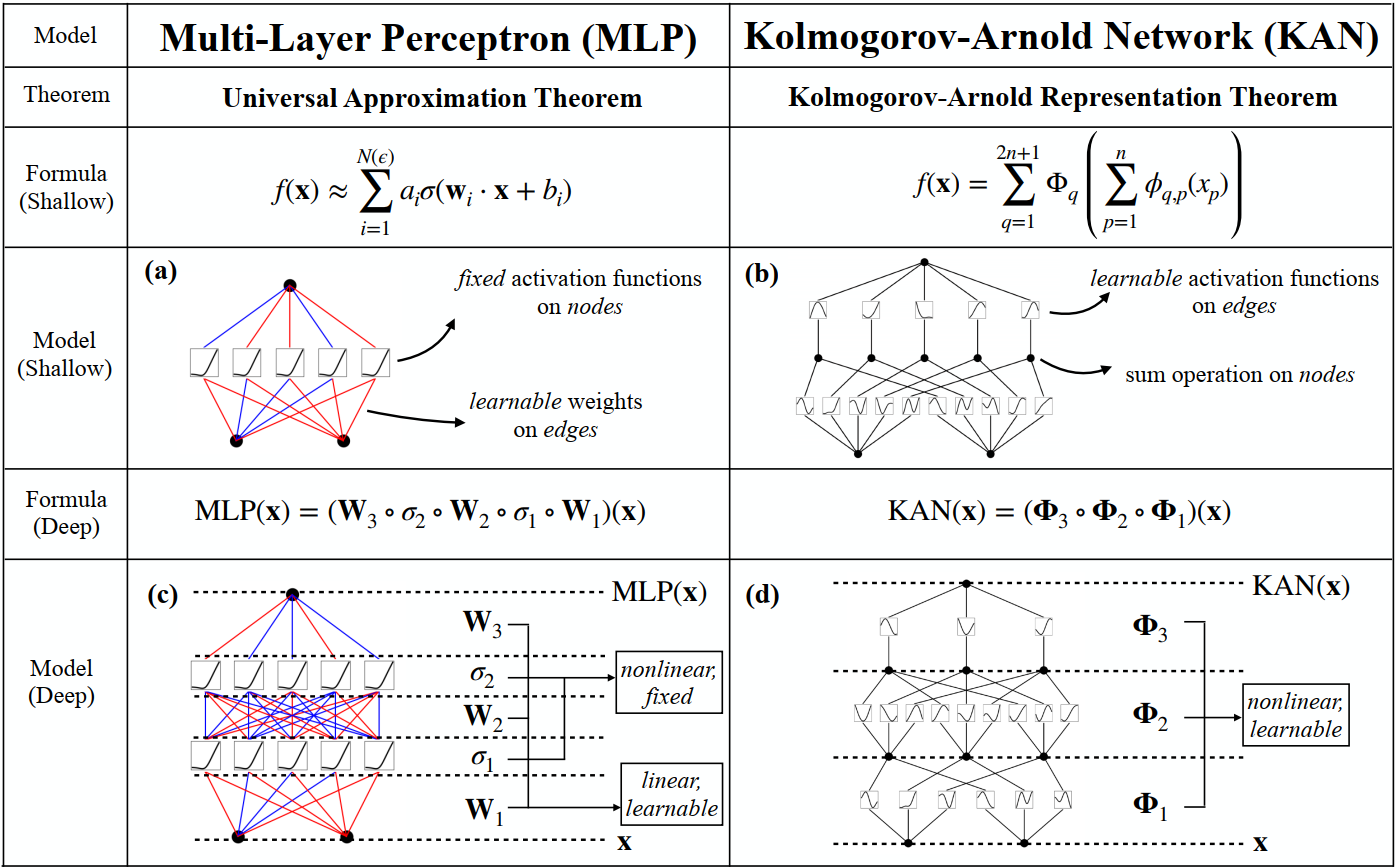
\includegraphics[width=0.9 \textwidth]{Figures/Fig1.png}
	\caption{Comparação entre as arquiteturas de uma \textit{Multi-Layer Perceptron} (\textit{MLP}) e uma \textit{Kolmogorov-Arnold Network} (\textit{KAN}) (LIU \textit{et al.} \cite{liu})}
	\label{fig:1}
\end{figure*}


Como todas as funções a serem aprendidas são funções univariadas, pode-se parametrizar cada função 1D como uma curva \textit{B-spline}, com coeficientes que podem ser aprendidos de funções de base \textit{B-spline} locais (Figura 2b). Desta maneira, tem-se um protótipo de \textit{KAN} cuja arquitetura é especificada exatamente pela Equação \ref{eq.1} e ilustrada na Figura 1b (com dimensão de entrada $n = 2$), compondo uma rede neural de duas camadas, cuja intermediária possui largura $2n+1$, e cujas funções de ativação são inseridas nas arestas ao invés de nós, onde a soma simples é realizada nos nós. A Figura \ref{fig:2} apresenta um esquema de como as funções de ativação fluem pela rede e como são parametrizadas como \textit{B-splines}.

\begin{figure*}[h!]
	\centering
	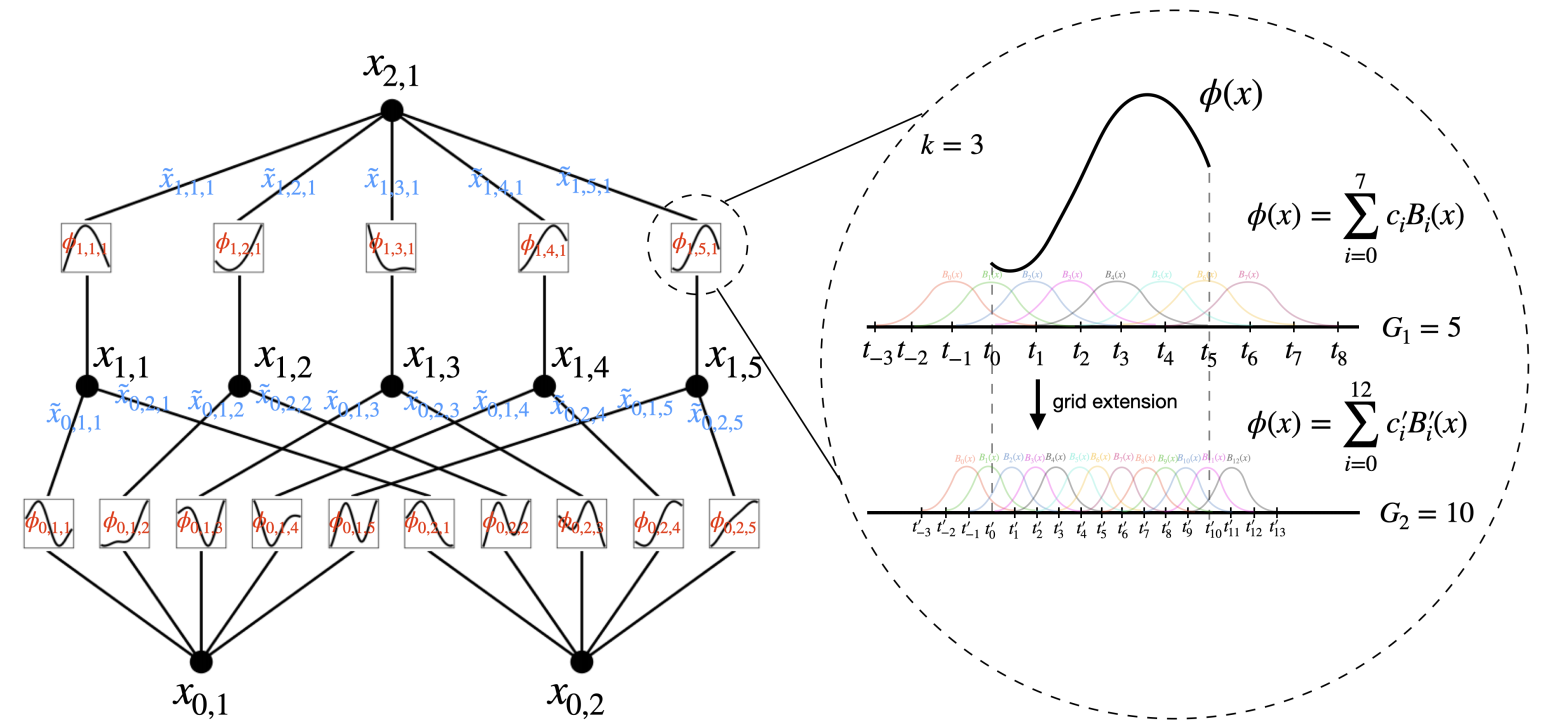
\includegraphics[width=0.9 \textwidth]{Figures/Fig2.png}
	\caption{Funções de ativação que fluem pela rede (a) e uma função de ativação parametrizada como \textit{B-spline}, que permite alternar entre \textit{grids} maiores e menores (b) (LIU \textit{et al.} \cite{liu}).}
	\label{fig:2}
\end{figure*}

Em termos de precisão, \textit{KANs} muito menores podem alcançar precisão comparável ou melhor do que \textit{MLPs} muito maiores no ajuste de dados e na resolução de Equações Diferenciais Parciais (\textit{Partial Differential Equations}, \textit{PDEs}), reduzindo o número parâmetros e possibilitando melhor generalização e interpretabilidade. Entretanto, geralmente o usuário vai desconhecer a arquitetura ótima de uma \textit{KAN} antes de resolver o problema. Desta maneira, Liu \textit{et al}. \cite{liu} propuseram uma abordagem que inicia pela proposição de uma \textit{KAN} grande, seguida de seu treino por meio de uma regularização esparsa e de um procedimento de poda, de modo que \textit{KANs} podadas são mais interpretáveis do que as não podadas. Esta abordagem é subdividida em quatro etapas: esparsificação, visualização, poda e simbolificação.

\section{METODOLOGIA}
\subsection{DESCRIÇÃO DOS \textit{DATASETS} E PRÉ-PROCESSAMENTO DOS DADOS}

O banco de dados \textit{Iris} contém um conjunto de 150 amostras com informações sobre quatro atributos, sendo \textit{sepal length, sepal width, petal length, petal width} e a variável de saída, a coluna \textit{species}, contendo os tipos de pétalas \textit{Setosa, Versicolor e Virginica}. As variáveis de entrada são numéricas, o banco de dados já é balanceado e não há dados faltantes, de modo que não é necessário empregar nenhum tratamento adicional aos dados.

O banco de dados \textit{Wine Quality} contém um conjunto de 4.898 amostras com informações sobre onze atributos, sendo \textit{fixed acidity, volatile acidity, citric acid, residual sugar, chlorides, free sulfur dioxide, total sulfur dioxide, density, pH, sulphates, color} e \textit{alcohol} as variáveis de entrada e \textit{quality} a variável de saída, contendo valores entre 0 e 10. Todas as variáveis são numéricas, a variável alvo é desbalanceada e não há dados faltantes, de modo que foi necessário realizar técnicas de oversampling.

O banco de dados \textit{Adult} contém um conjunto de 48.842 amostras com informações sobre quatorze atributos, sendo \textit{age, workclass, fnlwgt, education, education-num, marital-status, occupation, relationship, race, sex, capital-gain, capital-loss, hours-per-week} e \textit{native-country} as variáveis de entrada e \textit{income} a variável de saída, cujo objetivo é prever se a renda de um indivíduo excede US\$ 50 mil/ano. Este \textit{dataset} contém variáveis numéricas e categóricas, não apresenta dados faltantes, de modo que foi aplicado \textit{one hot encoder} nas variáveis categóricas, possibilitando tratar todo o conjunto de dados como numérico.

O banco de dados \textit{Brest Cancer Winsconsin} contém um conjunto de 569 amostras com informações sobre dez atributos, sendo \textit{radius, texture, perimeter, area, smoothness, compactness, concavity, concave points, symmetry} e \textit{fractal dimension} esses atributos. Como foram computadas em cada imagem a média, o erro padrão e o pior/maior (média dos três maiores valores) para cada variável, este \textit{dataset} na verdade apresenta trinta variáveis de entrada, sendo \textit{ID number} e \textit{diagnosis} as demais variáveis dos dados, podendo esta última representar um câncer benigno ou maligno. As variáveis de entrada são numéricas, o banco de dados já é balanceado e não há dados faltantes, de modo que não é necessário empregar nenhum tratamento adicional aos dados.

O banco de dados \textit{Heart Disease}, por sua vez, contém um conjunto de 303 amostras com informações sobre treze atributos, sendo \textit{age, sex, cp, trestbps, chol, fbs, restecg, thalach, exang, oldpeak, slope, ca} e \textit{thal} as variáveis de entrada, enquanto \textit{num} é a variável de saída, que indica o diagnóstico de doença cardíaca. Este \textit{dataset} contém variáveis numéricas e categóricas, além de haver dados faltantes, de modo foi necessário realizar um \textit{simpleimputer}. A variável alvo também está desbalanceada.

O banco de dados \textit{Rain in Australia} possui 145.000 amostras e informações associadas a 22 colunas de entrada. A variável de resposta seria \textit{RainTomorrow}, indicando se haveria ou não chuva no dia seguinte. Este \textit{dataset} contém variáveis numéricas e categóricas, além de haver dados faltantes, para contornar esses problemas foi utilizado o InterativeImputer do \textit{sklearn}, numa tentativa de lidar com os dados faltantes levando em consideração o grande grau de correlação entre as variáveis. Para lidar com as variáveis categóricas, os valores faltantes foram preenchidos randomicamente de acordo com a distribuição de probabilidade.

O banco de dados \textit{Spotify Tracks} contém 114.000 amostras e informações associadas a 19 variáveis de entrada. A variável resposta seria a coluna \textit{track\_genre}, composta por 115 categorias. Dentre as 19 colunas de entrada, todas aquelas que possuíam variáveis categóricas foram removidas (i.e.: \textit{track\_id, artists, album\_name, track\_name, key, liveness, mode, explicit, time\_signature}). Destarte, as colunas restantes para possibilitar o treinamento dos modelos foram \textit{popularity, duration\_ms, danceability, energy, loudness, speechiness, acousticness, instrumentalness, valence} e tempo. Não foi necessário eliminar nenhuma das 114.000 amostras, pois não haviam dados faltantes no conjunto de dados.

\subsection{TREINAMENTO E VALIDAÇÃO DOS MODELOS}
Considerando um determinado valor de \textit{seed}, para assegurar que os modelos de aprendizado fossem executados nas mesmas partições, os dados foram divididos em conjuntos de treinamento (80\%) e teste (20\%). Cada um destes conjuntos é composto por suas respectivas variáveis de entrada (X) e saída (y), sendo empregados em seguida no \textit{pipeline} de treinamento de cada modelo de aprendizado. Para minimizar o efeito da diferença de unidades entre as colunas, os dados do conjunto X de treinamento foram padronizados (\textit{scaling}) e transformados, transformação também aplicada nos conjuntos X de validação e teste, evitando assim um possível sobreajustamento.

Foi efetuada uma comparação quanto ao desempenho dos algoritmos \textit{k-NN, LVQ, SVM, DT, RF, MLP} e uma versão \textit{stacking} destes, além da avaliação do desempenho de uma rede neural \textit{KAN}. Para possibilitar uma otimização dos hiperparâmetros destes modelos de aprendizado, foi empregada uma estratégia \textit{grid search} com validação cruzada em 10 \textit{folds}, considerando a recuperação das métricas \textit{accuracy, precision, recall, F1} e \textit{Auc-ROC}. Desta forma, seria possível identificar para cada algoritmo qual configuração de hiperparâmetros resultaria em um menor erro. Neste âmbito, a Tabela \ref{tab:1} apresenta os conjuntos de hiperparâmetros testados para cada modelo de classificação.

\begin{table}[h!]
	\caption{Conjuntos de hiperparâmetros testados para cada modelo de classificação}
	\label{tab:1}
	\begin{tabular}{lllll}
		\cline{1-2}
		\textit{k-NN}      & \begin{tabular}[c]{@{}l@{}}n neighbors = range(1, 50); \\ metric = Euclidean, Manhattan;\end{tabular}                                                                                                                                                                  &  &  & \\ \cline{1-2}
		\textit{LVQ:}      & \begin{tabular}[c]{@{}l@{}}prototype n per class = range(1, 4); \\ distance type = Euclidean, Manhattan e Chebyshev; \\ solver params = (max runs = 5; \\ step size = 0.1, 0.5 e 1.0);\end{tabular}                                                                    &  &  & \\ \cline{1-2}
		\textit{SVM:}      & \begin{tabular}[c]{@{}l@{}}C = 0.1, 1; \\ gamma = 0.1, 1; \\ kernel = RBF, Sigmoid;\end{tabular}                                                                                                                                                                       &  &  & \\ \cline{1-2}
		\textit{DT:}       & \begin{tabular}[c]{@{}l@{}}criterion = Gini e entropy; \\ max depth = range(1, 10); \\ min samples split = range(2, 10); \\ min samples leaf = range(1, 10);\end{tabular}                                                                                              &  &  & \\ \cline{1-2}
		\textit{RF:}       & \begin{tabular}[c]{@{}l@{}}n estimators = 10, 20, 30 e 50; \\ criterion = Gini e entropy; \\ max depth = range(1, 6); \\ min samples split = range(2, 6); \\ min samples leaf = range(1, 6);\end{tabular}                                                              &  &  & \\ \cline{1-2}
		\textit{MLP:}      & \begin{tabular}[c]{@{}l@{}}hidden layer sizes = (50,), (100,), (50, 50), (100, 100); \\ activation = Tanh e ReLU; \\ solver = SGD e Adam; \\ alpha = 0.0001 e 0.05; \\ learning rate = constant e adaptive;\end{tabular}                                               &  &  & \\ \cline{1-2}
		\textit{Stacking:} & \begin{tabular}[c]{@{}l@{}}Nível 1: estimators = k-NN, LVQ, DT, ANN e RF \\ com conjuntos de hiperparâmetros otimizados \\por meio do grid search e da validaçãao cruzada; \\ Nível 2: final estimator = LogisticRegression\\ (max iter = 2000), cv = 10;\end{tabular} &  &  & \\ \cline{1-2}
		\textit{KAN:}      & \begin{tabular}[c]{@{}l@{}}Input dimension = Associado ao dataset;\\ Layer = 1;\\ Neurons = 20;\\ Grid = 10;\\ k = 4\end{tabular}                                                                                                                                      &  &  & \\ \cline{1-2}
	\end{tabular}
\end{table}

O número máximo de iterações de cada modelo de aprendizado foi determinado com 1.500 iterações, com exceção do nível 2 do modelo \textit{stacking}, onde foram consideradas 2.000 iterações em um modelo de regressão logística. Uma vez que as configurações ideais resultaram em um melhor modelo para o conjunto de treinamento, seria verificado ainda o desempenho deste modelo no conjunto de validação.
Já em relação ao ajuste dos hiperparâmetros do modelo \textit{KAN}, não foi possível realizar experimentos suficientes para otimizá-los. Ao passo que o \textit{Input\_dimension} e o \textit{Output\_dimension} estão associados aos \textit{datasets} sendo experimentados, inserir um número de neurônios maior que 20 inviabilizava a execução do algoritmo. Não foi testado também o efeito que um maior número de camadas exerceria na capacidade do algoritmo. O parâmetro \textit{k}, por fim, é a ordem polinomial do polinômio que se está tentando aproximar. De antemão, antes mesmo de apresentar os resultados, já sugerimos que é necessário que mais testes sejam efetuados para que seja possível explorar o potencial do modelo.

\subsection{FLUXOGRAMA DE EXECUÇÃO}

A Figura \ref{fig:3} apresenta o fluxograma executado no treinamento e teste de cada modelo de aprendizagem aplicado a cada \textit{dataset}.

\begin{figure*}
	\centering
	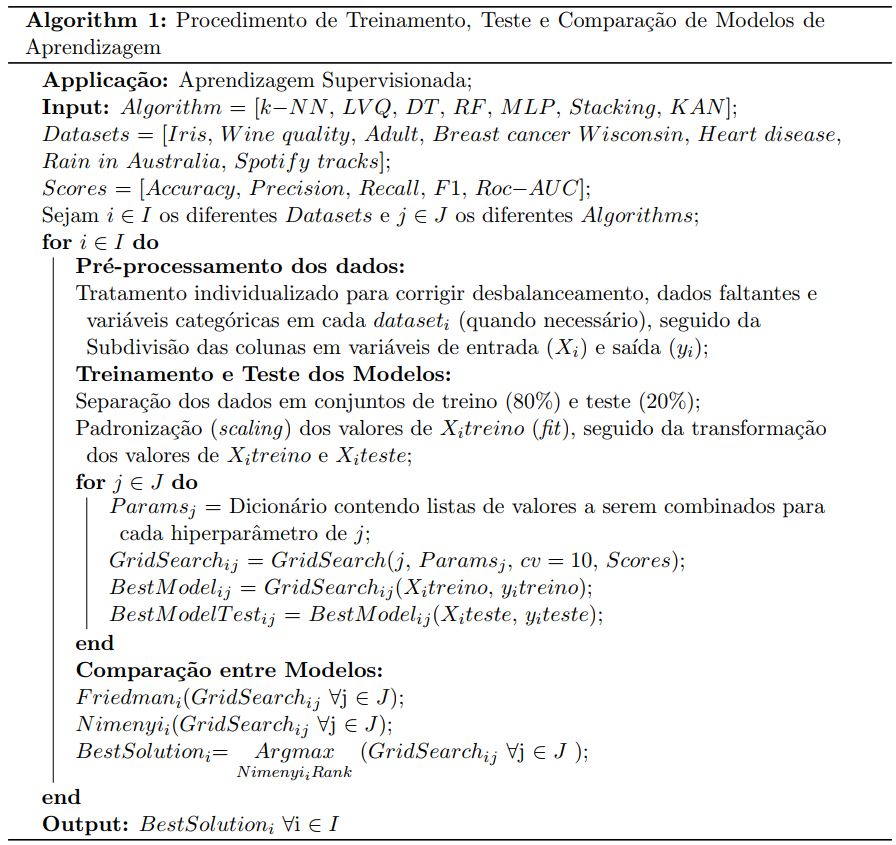
\includegraphics[width=0.7 \textwidth]{Figures/Fig3.png}
	\caption{Fluxograma da execução de treinamento e teste}
	\label{fig:3}
\end{figure*}

\subsection{FERRAMENTAS COMPUTACIONAIS}

Os experimentos foram conduzidos em \textit{Python}, sendo empregadas as bibliotecas \textit{Numpy}, {Pandas} e \textit{Scikit-Learning} para efetuar o tratamento dos dados (\textit{train test split, GridSearchCV}, etc). Quanto à implementação dos modelos de aprendizado, foram usadas também bibliotecas do \textit{Scikit-Learning} (\textit{KNeighborsClassifier, GLVQ, DecisionTreeClassifier, MLPClassifier, RandomForestClassifier} e \textit{StackingClassifier}). As métricas empregadas para avaliar os modelos também foram implementadas a partir de bibliotecas do \textit{Scikit-Learning} (\textit{make\_scorer, recall\_score, f1\_score, accuracy\_score, precision\_score} e \textit{roc\_auc\_score}).

Foram empregados 3 computadores: o primeiro com processador Intel i5 de 7ª geração, 12Gb de memoria RAM e sistema operacional Windows (64bits); o segundo com processador AMD Ryzen 5 3600 6-Core, 16Gb da memoria RAM e sistema operacional Windows (64bits); enquanto o terceiro contém processador i7 de 11 geração com 16 gb de memoria ram e sistema operacional Windows 11 (64bits). Esta divisão se fez necessária, uma vez que não haveria tempo hábil para executar todos os experimentos em uma única máquina.


\section{RESULTADOS E DISCUSSÃO}

Nesta seção são apresentados os resultados dos experimentos efetuados em cada \textit{dataset}, considerando o desempenho dos oito classificadores nos conjuntos de validação cruzada e teste em cada \textit{dataset}.

\subsection{IRIS DATASET}

Após a aplicação do \textit{grid search} com validação cruzada em 10 \textit{folds} no conjunto de treinamento do \textit{Iris Dataset}, a Tabela \ref{tab:2} apresenta os melhores hiperparâmetros verificados para cada modelo de classificação, ao passo que a Tabela \ref{tab:3} apresenta as métricas obtidas nestes dados. A Tabela \ref{tab:4}, por sua vez, apresenta as métricas obtidas no conjunto de testes do \textit{Iris Dataset}.

\begin{table}[h!]
	\caption{Melhores hiperparâmetros nos conjuntos de validação cruzada do Iris Dataset}
	\label{tab:2}
	\begin{tabular}{ l l }
		\hline
		\textit{k-NN:} & n\_neighbors = 10; metric = Euclidean;                     \\
		\hline
		\textit{LVQ:}  & prototype\_n\_per\_class = 3; distance\_type = Euclidean;  \\  & solver\_params = (max\_runs = 5; step\_size = 1.0);\\
		\hline
		\textit{SVM:}  & C = 1; gamma = 0.1; kernel = Sigmoid;                      \\
		\hline
		\textit{DT:}   & criterion = Gini; max\_depth = 3; min\_samples\_split = 2; \\  & min\_samples\_leaf = 3;\\
		\hline
		\textit{RF:}   & n\_estimators = 10; criterion = Gini; max\_depth = 2;      \\  & min\_samples\_split = 2; min\_samples\_leaf = 3;\\
		\hline
		\textit{MLP:}  & hidden\_layer\_sizes = (50, 50); activation = Tanh;        \\  & solver = Adam; alpha = 0.0001; learning\_rate = constant;\\
		\hline
	\end{tabular}
\end{table}

\begin{table}[h!]
	\caption{Desempenho na Validação cruzada - Iris Dataset}
	\label{tab:3}
	\begin{threeparttable}
		\begin{tabular}{lccccc}
			\hline
			\multicolumn{6}{c}{\textit{\textbf{Iris Dataset - Validação Cruzada}}}                                                                                                                               \\
			\multicolumn{1}{l|}{\textit{\textbf{Classificador}}} & \textit{\textbf{Accuracy}} & \textit{\textbf{Recall}}  & \textit{\textbf{F1}}      & \textit{\textbf{Precision}} & \textit{\textbf{Auc\_ROC}} \\ \hline
			\multicolumn{1}{l|}{\textit{k-NN}}                   & \cellcolor{lightgray}0.97  & \cellcolor{lightgray}0.97 & 0.96                      & \cellcolor{lightgray}0.97   & 0.98                       \\
			\multicolumn{1}{l|}{\textit{LVQ}}                    & 0.93                       & 0.93                      & 0.92                      & 0.94                        & 0.99                       \\
			\multicolumn{1}{l|}{\textit{SVM}}                    & \cellcolor{lightgray}0.97  & 0.96                      & \cellcolor{lightgray}0.97 & \cellcolor{lightgray}0.97   & \cellcolor{lightgray}1.00  \\
			\multicolumn{1}{l|}{\textit{DT}}                     & 0.95                       & 0.95                      & 0.95                      & 0.93                        & 0.97                       \\
			\multicolumn{1}{l|}{\textit{RF}}                     & 0.93                       & 0.93                      & 0.92                      & 0.95                        & 0.99                       \\
			\multicolumn{1}{l|}{\textit{MLP}}                    & 0.96                       & 0.96                      & 0.96                      & \cellcolor{lightgray}0.97   & \cellcolor{lightgray}1.00  \\
			\multicolumn{1}{l|}{\textit{Stacking}}               & 0.96                       & 0.96                      & 0.96                      & \cellcolor{lightgray}0.97   & \cellcolor{lightgray}1.00  \\
			\multicolumn{1}{l|}{\textit{KAN}}                    & 0.94                       & 0.95                      & 0.94                      & 0.94                        &                            \\
			\hline
		\end{tabular}
		\begin{tablenotes}\footnotesize
			\item[*] As células hachuradas contém os melhores desempenhos.
		\end{tablenotes}
	\end{threeparttable}
\end{table}

\begin{table}[h!]
	\caption{Desempenho no Teste - Iris Dataset}
	\label{tab:4}
	\begin{threeparttable}
		\begin{tabular}{lccccc}
			\hline
			\multicolumn{6}{c}{\textit{\textbf{Iris Dataset - Teste}}}                                                                                                                                           \\
			\multicolumn{1}{l|}{\textit{\textbf{Classificador}}} & \textit{\textbf{Accuracy}} & \textit{\textbf{Recall}}  & \textit{\textbf{F1}}      & \textit{\textbf{Precision}} & \textit{\textbf{Auc\_ROC}} \\ \hline
			\multicolumn{1}{l|}{\textit{k-NN}}                   & 0.97                       & 0.97                      & 0.97                      & 0.97                        & 0.99                       \\
			\multicolumn{1}{l|}{\textit{LVQ}}                    & \cellcolor{lightgray}1.00  & \cellcolor{lightgray}1.00 & \cellcolor{lightgray}1.00 & \cellcolor{lightgray}1.00   & \cellcolor{lightgray}1.00  \\
			\multicolumn{1}{l|}{\textit{SVM}}                    & \cellcolor{lightgray}1.00  & \cellcolor{lightgray}1.00 & \cellcolor{lightgray}1.00 & \cellcolor{lightgray}1.00   & \cellcolor{lightgray}1.00  \\
			\multicolumn{1}{l|}{\textit{DT}}                     & 0.93                       & 0.95                      & 0.93                      & 0.93                        & \cellcolor{lightgray}1.00  \\
			\multicolumn{1}{l|}{\textit{RF}}                     & 0.97                       & 0.97                      & 0.97                      & 0.96                        & \cellcolor{lightgray}1.00  \\
			\multicolumn{1}{l|}{\textit{MLP}}                    & \cellcolor{lightgray}1.00  & \cellcolor{lightgray}1.00 & \cellcolor{lightgray}1.00 & \cellcolor{lightgray}1.00   & \cellcolor{lightgray}1.00  \\
			\multicolumn{1}{l|}{\textit{Stacking}}               & 0.97                       & 0.97                      & 0.97                      & 0.96                        & \cellcolor{lightgray}1.00  \\
			\multicolumn{1}{l|}{\textit{KAN}}                    & 0.97                       & 0.97                      & 0.97                      & 0.96                        &                            \\
			\hline
		\end{tabular}
		\begin{tablenotes}\footnotesize
			\item[*] As células hachuradas contém os melhores desempenhos.
		\end{tablenotes}
	\end{threeparttable}
\end{table}

Tanto nos conjuntos de treinamento quanto de teste, todos os classificadores apresentaram resultados satisfatórios. Em relação à validação cruzada, os piores resultados foram obtidos pelos \textit{LVQ} e \textit{RF}, ao passo que os melhores resultados foram obtidos pelos \textit{k-NN} e \textit{SVM}. Já no conjunto de teste, o pior desempenho foi o do classificador \textit{DT}, ao passo que os classificadores \textit{LVQ}, \textit{SVM} e \textit{MLP} atingiram os valores máximos para todas as métricas averiguadas. O classificador \textit{KAN} apresentou um desempenho mediano no \textit{Iris dataset}.

Em relação ao teste de Friedman, a única métrica em que foi possível rejeitar a hipótese nula foi a \textit{Auc\_ROC}, indicando que havia uma diferença estatística entre os classificadores durante a validação cruzada. Não foi possível calcular esta métrica para o \textit{KAN}, de modo que o teste de Nemenyi foi aplicado nos demais resultados. Visto que muitos classificadores apresentaram desempenhos semelhantes, onde muitos \textit{folds} atingem a nota máxima, a implementação usada do \textit{Auc\_ROC} não foi capaz de criar um ranking adequado. Ela atribui melhor posição ao classificador verificado primeiro, mesmo que este tenha uma nota semelhante aos demais, fato verificado em diferentes testes, de modo que o teste não foi conclusivo para o \textit{Iris dataset}.

\subsection{WINE QUALITY DATASET}

Após a aplicação do \textit{grid search} com validação cruzada em 10 \textit{folds} no conjunto de treinamento do \textit{Wine Quality Dataset} exibe-se na Tabela \ref{tab:5} os melhores hiperparâmetros verificados para cada modelo de classificação, ao passo que a Tabela \ref{tab:6} apresenta as métricas obtidas nestes dados. A Tabela \ref{tab:7}, por sua vez, apresenta as métricas obtidas no conjunto de testes do \textit{Wine Quality Dataset}.

\begin{table}[h!]
	\caption{Melhores hiperparâmetros nos conjuntos de validação cruzada do Wine Quality Dataset}
	\label{tab:5}
	\begin{tabular}{ l l }
		\hline
		\textit{k-NN:} & n\_neighbors = 1; metric = Manhattan;                         \\
		\hline
		\textit{LVQ:}  & prototype\_n\_per\_class = 3; distance\_type = Euclidean;     \\  & solver\_params = (max\_runs = 5; step\_size = 0,5);\\
		\hline
		\textit{SVM:}  & C = 1; gamma = 1; kernel = rbf;                               \\
		\hline
		\textit{DT:}   & criterion = entropy; max\_depth = 9; min\_samples\_split = 3; \\  & min\_samples\_leaf = 1;\\
		\hline
		\textit{RF:}   & n\_estimators = 50; criterion = entropy; max\_depth = 5;      \\  & min\_samples\_split = 2; min\_samples\_leaf = 4;\\
		\hline
		\textit{MLP:}  & hidden\_layer\_sizes = (100, 100); activation = tanh;         \\  & solver = adam; alpha = 0.0001; learning\_rate = adaptive;\\
		\hline
	\end{tabular}
\end{table}

\begin{table}[h!]
	\caption{Desempenho na Validação cruzada - Wine Quality Dataset}
	\label{tab:6}
	\begin{threeparttable}
		\begin{tabular}{lccccc}
			\hline
			\multicolumn{6}{c}{\textit{\textbf{Wine Quality Dataset - Validação cruzada}}}                                                                                                                         \\
			\multicolumn{1}{l|}{\textit{\textbf{Classificador}}} & \textit{\textbf{Accuracy}} & \textit{\textbf{Recall}}   & \textit{\textbf{F1}}       & \textit{\textbf{Precision}} & \textit{\textbf{Auc\_ROC}} \\ \hline
			\multicolumn{1}{l|}{\textit{k-NN}}                   & 0.906                      & 0.906                      & 0.903                      & 0.902                       & 0.945                      \\
			\multicolumn{1}{l|}{\textit{LVQ}}                    & 0.454                      & 0.454                      & 0.425                      & 0.432                       & 0.795                      \\
			\multicolumn{1}{l|}{\textit{SVM}}                    & 0.893                      & 0.894                      & 0.892                      & 0.891                       & 0.987                      \\
			\multicolumn{1}{l|}{\textit{DT}}                     & 0.715                      & 0.716                      & 0.712                      & 0.712                       & 0.929                      \\
			\multicolumn{1}{l|}{\textit{RF}}                     & 0.636                      & 0.636                      & 0.616                      & 0.618                       & 0.901                      \\
			\multicolumn{1}{l|}{\textit{MLP}}                    & 0.904                      & 0.904                      & 0.900                      & 0.900                       & 0.976                      \\
			\multicolumn{1}{l|}{\textit{Stacking}}               & \cellcolor{lightgray}0.922 & \cellcolor{lightgray}0.923 & \cellcolor{lightgray}0.922 & \cellcolor{lightgray}0.922  & \cellcolor{lightgray}0.990 \\
			\multicolumn{1}{l|}{\textit{KAN}}                    & 0,143
			                                                     & 0,141
			                                                     & 0,035
			                                                     & 0,02
			                                                     & -                                                                                                                                               \\
			\hline
		\end{tabular}
		\begin{tablenotes}\footnotesize
			\item[*] As células hachuradas contém os melhores desempenhos.
		\end{tablenotes}
	\end{threeparttable}
\end{table}

\begin{table}[h!]
	\caption{Desempenho no Teste - Wine Quality Dataset}
	\label{tab:7}
	\begin{threeparttable}
		\begin{tabular}{lccccc}
			\hline
			\multicolumn{6}{c}{\textit{\textbf{Wine Quality Dataset - Teste}}}                                                                                                                                     \\
			\multicolumn{1}{l|}{\textit{\textbf{Classificador}}} & \textit{\textbf{Accuracy}} & \textit{\textbf{Recall}}   & \textit{\textbf{F1}}       & \textit{\textbf{Precision}} & \textit{\textbf{Auc\_ROC}} \\ \hline
			\multicolumn{1}{l|}{\textit{k-NN}}                   & 0.916                      & 0.915                      & 0.912                      & 0.913                       & 0.951                      \\
			\multicolumn{1}{l|}{\textit{LVQ}}                    & 0.468                      & 0.468                      & 0.439                      & 0.437                       & 0.795                      \\
			\multicolumn{1}{l|}{\textit{SVM}}                    & 0.908                      & 0.907                      & 0.905                      & 0.904                       & 0.989                      \\
			\multicolumn{1}{l|}{\textit{DT}}                     & 0.714                      & 0.711                      & 0.710                      & 0.711                       & 0.931                      \\
			\multicolumn{1}{l|}{\textit{RF}}                     & 0.633                      & 0.631                      & 0.612                      & 0.616                       & 0.901                      \\
			\multicolumn{1}{l|}{\textit{MLP}}                    & 0.914                      & 0.913                      & 0.910                      & 0.910                       & 0.979                      \\
			\multicolumn{1}{l|}{\textit{Stacking}}               & \cellcolor{lightgray}0.936 & \cellcolor{lightgray}0.935 & \cellcolor{lightgray}0.935 & \cellcolor{lightgray}0.934  & \cellcolor{lightgray}0.992 \\
			\multicolumn{1}{l|}{\textit{KAN}}                    & 0.14                       & 0.02                       & 0.14                       & 0.035                       & -                          \\
			\hline
		\end{tabular}
		\begin{tablenotes}\footnotesize
			\item[*] As células hachuradas contém os melhores desempenhos.
		\end{tablenotes}
	\end{threeparttable}
\end{table}

De toda a base de dados somente a coluna \textit{color} foi excluída da análise num primeiro momento, ao passo que as outras 11 colunas são valores reais. Na etapa de treino os classificadores que apresentaram melhor comportamento foram \textit{k-NN, MLP} e \textit{stacking}. O fato dos dados estarem próximos uns dos outros e a maneira como os algoritmos executam as aproximações beneficiaram \textit{k-NN} e \textit{MLP}. Em contrapartida, no treinamento os piores desempenhos foram do \textit{KAN} e \textit{LVQ}.

Na etapa de teste, conforme visto na tabela \ref{tab:7}, o melhor classificador  foi \textit{Stacking}. De modo geral, o desempenho no teste foi bom apenas para alguns algoritmos, como \textit{k-NN, SVM, MLP} e \textit{Stacking}. Já para \textit{LVQ, DT, RF e KAN} o desempenho não foi bom. Um fator que pode ter influenciado na queda de performance, é o desbalanceamento do banco de dados, que apesar de ter sido contornado com \textit{RandomOverSampler} não foi favorecido pelos algoritmos.

Para o balanceamento não foi viável técnicas de \textit{under sampling}, pois algumas classificações de qualidade tinham poucos dados, especificamente na casa de unidades, enquanto outras estavam na casa de milhar (i.e.: a nota 9 aparece em 5 ocorrências, enquanto a nota 6 aparece 2836 vezes). Deste modo, técnicas de \textit{over sampling} foram as alternativas possíveis. Entre \textit{Synthetic Minority Over-sampling Technique (SMOTE)} e \textit{RandomOverSampler}, esta apresentou melhores resultados e comportamento no balanceamento.

O classificador \textit{KAN} passou por mais testes em que foram alterados o número de neurônios na camada oculta, de 10 passou para 19 neurônios. Contudo, obteve-se os mesmos resultados da tabela \ref{tab:7}.

Do teste de Friedman foi verificados que os valores de \textit{p} para \textit{Accuracy, Recall, F1 Score, Precision} e \textit{Roc-Auc} foram menores que 0,05 e proximos de 0, logo há evidências estatísticas de que existe ao menos uma diferença significativa entre os grupos testados. Por fim, foi aplicado o teste de \textit{Nimenyi} em que os menores rankings médios, portanto, melhor avaliados foram: \textit{Stacking, SVM} e \textit{MLP}.


\subsection{ADULT DATASET}

Após a aplicação do \textit{grid search} com validação cruzada em 10 \textit{folds} no conjunto de treinamento do \textit{Adult Dataset}, a Tabela \ref{tab:8} apresenta os melhores hiperparâmetros verificados para cada modelo de classificação, ao passo que a Tabela \ref{tab:9} apresenta as métricas obtidas nestes dados. A Tabela \ref{tab:10}, por sua vez, apresenta as métricas obtidas no conjunto de testes do \textit{Adult Dataset}.

\begin{table}[h!]
	\caption{Melhores hiperparâmetros nos conjuntos de validação cruzada do Adult Dataset}
	\label{tab:8}
	\begin{tabular}{ l l }
		\hline
		\textit{k-NN:} & n\_neighbors = 17; metric = Euclidean;                     \\
		\hline
		\textit{LVQ:}  & prototype\_n\_per\_class = 3; distance\_type = Euclidean;  \\  & solver\_params = (max\_runs = 5; step\_size = 0.1);\\
		\hline
		\textit{SVM:}  & C = 1; gamma = 0.1; kernel = RBF;                          \\
		\hline
		\textit{DT:}   & criterion = Gini; max\_depth = 9; min\_samples\_split = 8; \\  & min\_samples\_leaf = 3;\\
		\hline
		\textit{RF:}   & n\_estimators = 30; criterion = entropy; max\_depth = 5;   \\  & min\_samples\_split = 2; min\_samples\_leaf = 4;\\
		\hline
		\textit{MLP:}  & hidden\_layer\_sizes = (50,); activation = Tanh;           \\  & solver = Adam; alpha = 0.05; learning\_rate = constant;\\
		\hline
	\end{tabular}
\end{table}

\begin{table}[h!]
	\caption{Desempenho na Validação cruzada - Adult Dataset}
	\label{tab:9}
	\begin{threeparttable}
		\begin{tabular}{lccccc}
			\hline
			\multicolumn{6}{c}{\textit{\textbf{Adult Dataset - Validação Cruzada}}}                                                                                                                              \\
			\multicolumn{1}{l|}{\textit{\textbf{Classificador}}} & \textit{\textbf{Accuracy}} & \textit{\textbf{Recall}}  & \textit{\textbf{F1}}      & \textit{\textbf{Precision}} & \textit{\textbf{Auc\_ROC}} \\ \hline
			\multicolumn{1}{l|}{\textit{k-NN}}                   & 0.84                       & 0.76                      & 0.77                      & 0.79                        & 0.89                       \\
			\multicolumn{1}{l|}{\textit{LVQ}}                    & 0.76                       & 0.51                      & 0.45                      & \cellcolor{lightgray}0.88   & 0.85                       \\
			\multicolumn{1}{l|}{\textit{SVM}}                    & \cellcolor{lightgray}0.86  & 0.77                      & 0.79                      & 0.82                        & 0.90                       \\
			\multicolumn{1}{l|}{\textit{DT}}                     & \cellcolor{lightgray}0.86  & \cellcolor{lightgray}0.78 & 0.79                      & 0.81                        & 0.90                       \\
			\multicolumn{1}{l|}{\textit{RF}}                     & 0.83                       & 0.68                      & 0.71                      & 0.82                        & 0.90                       \\
			\multicolumn{1}{l|}{\textit{MLP}}                    & \cellcolor{lightgray}0.86  & \cellcolor{lightgray}0.78 & 0.79                      & 0.81                        & 0.91                       \\
			\multicolumn{1}{l|}{\textit{Stacking}}               & \cellcolor{lightgray}0.86  & \cellcolor{lightgray}0.78 & \cellcolor{lightgray}0.80 & 0.82                        & \cellcolor{lightgray}0.92  \\
			\multicolumn{1}{l|}{\textit{KAN}}                    & 0.84                       & 0.74                      & 0.76                      & 0.79                        &                            \\
			\hline
		\end{tabular}
		\begin{tablenotes}\footnotesize
			\item[*] As células hachuradas contém os melhores desempenhos.
		\end{tablenotes}
	\end{threeparttable}
\end{table}

\begin{table}[h!]
	\caption{Desempenho no Teste - Adult Dataset}
	\label{tab:10}
	\begin{threeparttable}
		\begin{tabular}{lccccc}
			\hline
			\multicolumn{6}{c}{\textit{\textbf{Adult Dataset - Teste}}}                                                                                                                                          \\
			\multicolumn{1}{l|}{\textit{\textbf{Classificador}}} & \textit{\textbf{Accuracy}} & \textit{\textbf{Recall}}  & \textit{\textbf{F1}}      & \textit{\textbf{Precision}} & \textit{\textbf{Auc\_ROC}} \\ \hline
			\multicolumn{1}{l|}{\textit{k-NN}}                   & 0.84                       & 0.77                      & 0.78                      & 0.79                        & 0.89                       \\
			\multicolumn{1}{l|}{\textit{LVQ}}                    & 0.76                       & 0.51                      & 0.45                      & \cellcolor{lightgray}0.88   & 0.85                       \\
			\multicolumn{1}{l|}{\textit{SVM}}                    & 0.86                       & 0.77                      & 0.80                      & 0.82                        & 0.90                       \\
			\multicolumn{1}{l|}{\textit{DT}}                     & 0.86                       & 0.78                      & 0.80                      & 0.81                        & 0.91                       \\
			\multicolumn{1}{l|}{\textit{RF}}                     & 0.84                       & 0.71                      & 0.74                      & 0.81                        & 0.90                       \\
			\multicolumn{1}{l|}{\textit{MLP}}                    & \cellcolor{lightgray}0.87  & \cellcolor{lightgray}0.79 & \cellcolor{lightgray}0.81 & 0.83                        & \cellcolor{lightgray}0.92  \\
			\multicolumn{1}{l|}{\textit{Stacking}}               & \cellcolor{lightgray}0.87  & \cellcolor{lightgray}0.79 & \cellcolor{lightgray}0.81 & 0.83                        & \cellcolor{lightgray}0.92  \\
			\multicolumn{1}{l|}{\textit{KAN}}                    & 0.86                       & 0.78                      & 0.80                      & 0.82                        &                            \\
			\hline
		\end{tabular}
		\begin{tablenotes}\footnotesize
			\item[*] As células hachuradas contém os melhores desempenhos.
		\end{tablenotes}
	\end{threeparttable}
\end{table}

Em relação à validação cruzada, os piores resultados foram obtidos pelo \textit{LVQ}, ao passo que os melhores resultados foram obtidos pelo classificador \textit{Stacking}. Já no conjunto de teste, o pior desempenho apresentado foi novamente o do \textit{LVQ}, ao passo que os classificadores \textit{MLP} e \textit{Stacking} apresentaram as melhores métricas. O classificador \textit{KAN} apresentou um desempenho próximo aos dos melhores classificadores no \textit{Adult dataset}.

Em relação ao teste de Friedman, em todas as métricas foi possível rejeitar a hipótese nula, indicando que havia uma diferença estatística entre os classificadores durante a validação cruzada. Portanto, o teste de Nemenyi foi aplicado a esses conjuntos de dados. O classificador \textit{MLP} esteve entre os dois melhores em todos os testes, ao passo que o \textit{KNN} esteve quatro vezes nas melhores colocações, seguido pelo \textit{LVQ}, que foi o primeiro colocado na métrica \textit{Auc\_ROC}. Em geral, o desempenho do \textit{KAN} foi mediano a baixo nestes testes, não sendo possível calcular seu desempenho para a métrica \textit{Auc\_ROC}.

\subsection{BREST CANCER WINSCONSIN DATASET}

Após a aplicação do \textit{grid search} com validação cruzada em 10 \textit{folds} no conjunto de treinamento do \textit{Breast Cancer Winsconsin Dataset}, a Tabela \ref{tab:11} apresenta os melhores hiperparâmetros verificados para cada modelo de classificação, ao passo que a Tabela \ref{tab:12} apresenta as métricas obtidas nestes dados. A Tabela \ref{tab:13}, por sua vez, apresenta as métricas obtidas no conjunto de testes do \textit{Breast Cancer Winsconsin Dataset}.

\begin{table}[h!]
	\caption{Melhores hiperparâmetros nos conjuntos de validação cruzada do Breast Cancer Winsconsin Dataset}
	\label{tab:11}
	\begin{tabular}{ l l }
		\hline
		\textit{k-NN:} & n\_neighbors = 3; metric = Manhattan;                         \\
		\hline
		\textit{LVQ:}  & prototype\_n\_per\_class = 3; distance\_type = Euclidean;     \\  & solver\_params = (max\_runs = 5; step\_size = 0.5);\\
		\hline
		\textit{SVM:}  & C = 1; gamma = 0.1; kernel = RBF;                             \\
		\hline
		\textit{DT:}   & criterion = entropy; max\_depth = 6; min\_samples\_split = 2; \\  & min\_samples\_leaf = 1;\\
		\hline
		\textit{RF:}   & n\_estimators = 10; criterion = Gini; max\_depth = 5;         \\  & min\_samples\_split = 3; min\_samples\_leaf = 1;\\
		\hline
		\textit{MLP:}  & hidden\_layer\_sizes = (50, 50); activation = ReLu;           \\  & solver = Adam; alpha = 0.0001; learning\_rate = adaptive;\\
		\hline
	\end{tabular}
\end{table}

\begin{table}[h!]
	\caption{Desempenho na Validação cruzada - Breast Cancer Winsconsin Dataset}
	\label{tab:12}
	\begin{threeparttable}
		\begin{tabular}{lccccc}
			\hline
			\multicolumn{6}{c}{\textit{\textbf{Breast Cancer Winsconsin Dataset - Validação cruzada}}}                                                                                                           \\
			\multicolumn{1}{l|}{\textit{\textbf{Classificador}}} & \textit{\textbf{Accuracy}} & \textit{\textbf{Recall}}  & \textit{\textbf{F1}}      & \textit{\textbf{Precision}} & \textit{\textbf{Auc\_ROC}} \\ \hline
			\multicolumn{1}{l|}{\textit{k-NN}}                   & 0.97                       & 0.97                      & 0.97                      & 0.97                        & 0.98                       \\
			\multicolumn{1}{l|}{\textit{LVQ}}                    & 0.94                       & 0.92                      & 0.93                      & 0.95                        & \cellcolor{lightgray}0.99  \\
			\multicolumn{1}{l|}{\textit{SVM}}                    & 0.96                       & 0.96                      & 0.95                      & 0.96                        & \cellcolor{lightgray}0.99  \\
			\multicolumn{1}{l|}{\textit{DT}}                     & 0.93                       & 0.93                      & 0.93                      & 0.93                        & 0.93                       \\
			\multicolumn{1}{l|}{\textit{RF}}                     & 0.95                       & 0.95                      & 0.95                      & 0.95                        & 0.98                       \\
			\multicolumn{1}{l|}{\textit{MLP}}                    & \cellcolor{lightgray}0.98  & \cellcolor{lightgray}0.98 & \cellcolor{lightgray}0.98 & 0.98                        & \cellcolor{lightgray}0.99  \\
			\multicolumn{1}{l|}{\textit{Stacking}}               & \cellcolor{lightgray}0.98  & \cellcolor{lightgray}0.98 & \cellcolor{lightgray}0.98 & \cellcolor{lightgray}0.99   & \cellcolor{lightgray}0.99  \\
			\multicolumn{1}{l|}{\textit{KAN}}                    & 0.96                       & 0.93                      & 0.93                      & 0.94                        &                            \\
			\hline
		\end{tabular}
		\begin{tablenotes}\footnotesize
			\item[*] As células hachuradas contém os melhores desempenhos.
		\end{tablenotes}
	\end{threeparttable}
\end{table}

\begin{table}[h!]
	\caption{Desempenho no Teste - Breast Cancer Winsconsin Dataset}
	\label{tab:13}
	\begin{threeparttable}
		\begin{tabular}{lccccc}
			\hline
			\multicolumn{6}{c}{\textit{\textbf{Breast Cancer Winsconsin Dataset - Teste}}}                                                                                                                       \\
			\multicolumn{1}{l|}{\textit{\textbf{Classificador}}} & \textit{\textbf{Accuracy}} & \textit{\textbf{Recall}}  & \textit{\textbf{F1}}      & \textit{\textbf{Precision}} & \textit{\textbf{Auc\_ROC}} \\ \hline
			\multicolumn{1}{l|}{\textit{k-NN}}                   & 0.97                       & 0.95                      & 0.96                      & 0.97                        & 0.97                       \\
			\multicolumn{1}{l|}{\textit{LVQ}}                    & 0.92                       & 0.89                      & 0.91                      & 0.94                        & \cellcolor{lightgray}0.99  \\
			\multicolumn{1}{l|}{\textit{SVM}}                    & 0.93                       & 0.93                      & 0.93                      & 0.92                        & \cellcolor{lightgray}0.99  \\
			\multicolumn{1}{l|}{\textit{DT}}                     & 0.94                       & 0.92                      & 0.93                      & 0.96                        & 0.95                       \\
			\multicolumn{1}{l|}{\textit{RF}}                     & 0.96                       & 0.96                      & 0.95                      & 0.96                        & 0.98                       \\
			\multicolumn{1}{l|}{\textit{MLP}}                    & \cellcolor{lightgray}0.98  & \cellcolor{lightgray}0.98 & 0.97                      & 0.98                        & \cellcolor{lightgray}0.99  \\
			\multicolumn{1}{l|}{\textit{Stacking}}               & \cellcolor{lightgray}0.98  & \cellcolor{lightgray}0.98 & \cellcolor{lightgray}0.98 & \cellcolor{lightgray}0.99   & \cellcolor{lightgray}0.99  \\
			\multicolumn{1}{l|}{\textit{KAN}}                    & 0.97                       & 0.96                      & 0.97                      & 0.98                        &                            \\
			\hline
		\end{tabular}
		\begin{tablenotes}\footnotesize
			\item[*] As células hachuradas contém os melhores desempenhos.
		\end{tablenotes}
	\end{threeparttable}
\end{table}

Tanto nos conjuntos de treinamento quanto de teste, todos os classificadores apresentaram resultados satisfatórios. Em relação à validação cruzada, os piores resultados foram obtidos pelos classificadores \textit{LVQ}, \textit{DT} e \textit{KAN}, ao passo que os melhores resultados foram obtidos pelos classificadores \textit{Stacking} e \textit{MLP}, respectivamente. Já no conjunto de teste, os piores desempenhos apresentados foram os do \textit{LVQ}, \textit{DT} e \textit{SVM} ao passo que os classificadores \textit{Stacking} e \textit{MLP} novamente apresentaram as melhores métricas, respectivamente. O classificador \textit{KAN} apresentou um desempenho próximo aos dos melhores classificadores no conjunto de testes do \textit{Breast Cancer Winsconsin dataset}.

Em relação ao teste de Friedman, em todas as métricas foi possível rejeitar a hipótese nula, indicando que havia uma diferença estatística entre os classificadores durante a validação cruzada. Portanto, o teste de Nemenyi foi aplicado a esses conjuntos de dados. Com exceção da métrica \textit{precision}, os classificadores \textit{Stacking} e \textit{MLP} foram o primeiro e o segundo colocados em todas as métricas, respectivamente. Em relação à métrica \textit{precision}, os melhores resultados foram obtidos pelo \textit{LVQ}, \textit{RF} e \textit{Stacking}, respectivamente. Em geral, o desempenho do \textit{KAN} foi baixo nestes testes, não sendo possível calcular seu desempenho para a métrica \textit{Auc\_ROC}.

\subsection{HEART DISEASE DATASET}

Após a aplicação do \textit{grid search} com validação cruzada em 10 \textit{folds} no conjunto de treinamento do \textit{Heart Disease Dataset}, a Tabela \ref{tab:14} apresenta os melhores hiperparâmetros verificados para cada modelo de classificação, ao passo que a Tabela \ref{tab:15} apresenta as métricas obtidas nestes dados. A Tabela \ref{tab:16}, por sua vez, apresenta as métricas obtidas no conjunto de testes do \textit{Heart Disease Dataset}.

\begin{table}[h!]
	\caption{Melhores hiperparâmetros nos conjuntos de validação cruzada do Heart Disease Dataset}
	\label{tab:14}
	\begin{tabular}{ l l }
		\hline
		\textit{k-NN:} & n\_neighbors = 4; metric = Euclidean;                         \\
		\hline
		\textit{LVQ:}  & prototype\_n\_per\_class = 3; distance\_type = Euclidean;     \\  & solver\_params = (max\_runs = 5; step\_size = 0.1);\\
		\hline
		\textit{SVM:}  & C = 1; gamma = 1; kernel = Sigmoid;                           \\
		\hline
		\textit{DT:}   & criterion = entropy; max\_depth = 8; min\_samples\_split = 2; \\  & min\_samples\_leaf = 2;\\
		\hline
		\textit{RF:}   & n\_estimators = 10; criterion = entropy; max\_depth = 5;      \\  & min\_samples\_split = 5; min\_samples\_leaf = 1;\\
		\hline
		\textit{MLP:}  & hidden\_layer\_sizes = (100, 100); activation = ReLu;         \\  & solver = SGD; alpha = 0.05; learning\_rate = constant;\\
		\hline
	\end{tabular}
\end{table}

\begin{table}[h!]
	\caption{Desempenho na Validação cruzada - Heart Disease Dataset}
	\label{tab:15}
	\begin{threeparttable}
		\begin{tabular}{lccccc}
			\hline
			\multicolumn{6}{c}{\textit{\textbf{Heart Disease Dataset - Validação cruzada}}}                                                                                                                      \\
			\multicolumn{1}{l|}{\textit{\textbf{Classificador}}} & \textit{\textbf{Accuracy}} & \textit{\textbf{Recall}}  & \textit{\textbf{F1}}      & \textit{\textbf{Precision}} & \textit{\textbf{Auc\_ROC}} \\ \hline
			\multicolumn{1}{l|}{\textit{k-NN}}                   & \cellcolor{lightgray}0.62  & 0.37                      & \cellcolor{lightgray}0.36 & \cellcolor{lightgray}0.36   &                            \\
			\multicolumn{1}{l|}{\textit{LVQ}}                    & 0.58                       & 0.33                      & 0.29                      & 0.29                        &                            \\
			\multicolumn{1}{l|}{\textit{SVM}}                    & 0.53                       & 0.31                      & 0.30                      & 0.31                        &                            \\
			\multicolumn{1}{l|}{\textit{DT}}                     & 0.55                       & 0.33                      & 0.31                      & 0.31                        &                            \\
			\multicolumn{1}{l|}{\textit{RF}}                     & 0.58                       & 0.31                      & 0.28                      & 0.28                        &                            \\
			\multicolumn{1}{l|}{\textit{MLP}}                    & 0.56                       & 0.34                      & 0.30                      & 0.27                        &                            \\
			\multicolumn{1}{l|}{\textit{Stacking}}               & 0.60                       & 0.31                      & 0.29                      & 0.31                        &                            \\
			\multicolumn{1}{l|}{\textit{KAN}}                    & 0.60                       & \cellcolor{lightgray}0.39 & 0.35                      & 0.35                        &                            \\
			\hline
		\end{tabular}
		\begin{tablenotes}\footnotesize
			\item[*] As células hachuradas contém os melhores desempenhos.
		\end{tablenotes}
	\end{threeparttable}
\end{table}

\begin{table}[h!]
	\caption{Desempenho no Teste - Heart Disease Dataset}
	\label{tab:16}
	\begin{threeparttable}
		\begin{tabular}{lccccc}
			\hline
			\multicolumn{6}{c}{\textit{\textbf{Heart Disease Dataset - Teste}}}                                                                                                                                  \\
			\multicolumn{1}{l|}{\textit{\textbf{Classificador}}} & \textit{\textbf{Accuracy}} & \textit{\textbf{Recall}}  & \textit{\textbf{F1}}      & \textit{\textbf{Precision}} & \textit{\textbf{Auc\_ROC}} \\ \hline
			\multicolumn{1}{l|}{\textit{k-NN}}                   & 0.54                       & 0.27                      & 0.23                      & 0.21                        & 0.64                       \\
			\multicolumn{1}{l|}{\textit{LVQ}}                    & 0.53                       & 0.29                      & 0.29                      & 0.30                        & 0.76                       \\
			\multicolumn{1}{l|}{\textit{SVM}}                    & 0.51                       & 0.32                      & 0.33                      & \cellcolor{lightgray}0.42   & 0.65                       \\
			\multicolumn{1}{l|}{\textit{DT}}                     & 0.43                       & 0.28                      & 0.27                      & 0.29                        & 0.62                       \\
			\multicolumn{1}{l|}{\textit{RF}}                     & 0.56                       & 0.29                      & 0.27                      & 0.30                        & 0.78                       \\
			\multicolumn{1}{l|}{\textit{MLP}}                    & 0.54                       & 0.34                      & 0.32                      & 0.32                        & 0.77                       \\
			\multicolumn{1}{l|}{\textit{Stacking}}               & \cellcolor{lightgray}0.57  & 0.33                      & 0.31                      & 0.29                        & \cellcolor{lightgray}0.79  \\
			\multicolumn{1}{l|}{\textit{KAN}}                    & 0.54                       & \cellcolor{lightgray}0.37 & \cellcolor{lightgray}0.36 & 0.36                        &                            \\
			\hline
		\end{tabular}
		\begin{tablenotes}\footnotesize
			\item[*] As células hachuradas contém os melhores desempenhos.
		\end{tablenotes}
	\end{threeparttable}
\end{table}

Em relação à validação cruzada, os melhores resultados foram obtidos pelos classificadores \textit{k-NN}, tendo o \textit{KAN} vencido os demais em relação à métrica \textit{Recall}. Já no conjunto de teste, os piores desempenhos apresentados foram os do \textit{k-NN}, sugerindo que o modelo teve \textit{overfitting} nos dados de treinamento, ao passo que os classificadores \textit{Stacking} e \textit{KAN} apresentaram as melhores métricas.

Em relação ao teste de Friedman, somente em relação à métrica \textit{Recall} foi possível rejeitar a hipótese nula, indicando que havia uma diferença estatística entre os classificadores durante a validação cruzada. Portanto, o teste de Nemenyi foi aplicado, indicando que os melhores classificadores aplicados ao \textit{Heart Disease dataset} eram o \textit{KAN} e o \textit{MLP}, respectivamente.
Novamente, não foi possível calcular o desempenho do \textit{KAN} para a métrica \textit{Auc\_ROC}.

\begin{table}[h!]
	\caption{Desempenho na Validação cruzada - Heart Disease Dataset}
	\label{tab:23}
	\begin{threeparttable}
		\begin{tabular}{lccccc}
			\hline
			\multicolumn{6}{c}{\textit{\textbf{Heart Disease Dataset - Validação cruzada}}}                                                                                                                 \\
			\multicolumn{1}{l|}{\textit{\textbf{Classificador}}} & \textit{\textbf{Accuracy}} & \textit{\textbf{Recall}}  & \textit{\textbf{F1}} & \textit{\textbf{Precision}} & \textit{\textbf{Auc\_ROC}} \\ \hline
			\multicolumn{1}{l|}{\textit{k-NN}}                   & \cellcolor{lightgray}0.62  & 0.37                      & 0.36                 & 0.36                        &                            \\
			\multicolumn{1}{l|}{\textit{LVQ}}                    & 0.58                       & 0.33                      & 0.29                 & 0.29                        &                            \\
			\multicolumn{1}{l|}{\textit{SVM}}                    & 0.53                       & 0.31                      & 0.29                 & 0.31                        &                            \\
			\multicolumn{1}{l|}{\textit{DT}}                     & 0.55                       & 0.33                      & 0.31                 & 0.31                        &                            \\
			\multicolumn{1}{l|}{\textit{RF}}                     & 0.58                       & 0.27                      & 0.25                 & 0.24                        &                            \\
			\multicolumn{1}{l|}{\textit{MLP}}                    & 0.56                       & 0.34                      & 0.30                 & 0.27                        &                            \\
			\multicolumn{1}{l|}{\textit{Stacking}}               & \cellcolor{lightgray}0.62  & 0.38                      & 0.36                 & \cellcolor{lightgray}0.38   &                            \\
			\multicolumn{1}{l|}{\textit{KAN}}                    & 0.60                       & \cellcolor{lightgray}0.39 & 0.35                 & 0.35                        &                            \\
			\hline
		\end{tabular}
		\begin{tablenotes}\footnotesize
			\item[*] As células hachuradas contém os melhores desempenhos.
		\end{tablenotes}
	\end{threeparttable}
\end{table}

\begin{table}[h!]
	\caption{Desempenho no Teste - Heart Disease Dataset}
	\label{tab:24}
	\begin{threeparttable}
		\begin{tabular}{lccccc}
			\hline
			\multicolumn{6}{c}{\textit{\textbf{Heart Disease Dataset - Teste}}}                                                                                                                                  \\
			\multicolumn{1}{l|}{\textit{\textbf{Classificador}}} & \textit{\textbf{Accuracy}} & \textit{\textbf{Recall}}  & \textit{\textbf{F1}}      & \textit{\textbf{Precision}} & \textit{\textbf{Auc\_ROC}} \\ \hline
			\multicolumn{1}{l|}{\textit{k-NN}}                   & 0.54                       & 0.27                      & 0.23                      & 0.21                        & 0.64                       \\
			\multicolumn{1}{l|}{\textit{LVQ}}                    & 0.53                       & 0.29                      & 0.29                      & 0.30                        & 0.76                       \\
			\multicolumn{1}{l|}{\textit{SVM}}                    & 0.49                       & 0.30                      & 0.29                      & 0.29                        & 0.79                       \\
			\multicolumn{1}{l|}{\textit{DT}}                     & 0.43                       & 0.28                      & 0.27                      & 0.29                        & 0.62                       \\
			\multicolumn{1}{l|}{\textit{RF}}                     & 0.53                       & 0.35                      & 0.35                      & 0.39                        & 0.76                       \\
			\multicolumn{1}{l|}{\textit{MLP}}                    & 0.54                       & 0.34                      & 0.32                      & 0.32                        & 0.77                       \\
			\multicolumn{1}{l|}{\textit{Stacking}}               & 0.53                       & 0.30                      & 0.29                      & 0.28                        & \cellcolor{lightgray}0.78  \\
			\multicolumn{1}{l|}{\textit{KAN}}                    & \cellcolor{lightgray}0.56  & \cellcolor{lightgray}0.39 & \cellcolor{lightgray}0.38 & \cellcolor{lightgray}0.38   &                            \\
			\hline
		\end{tabular}
		\begin{tablenotes}\footnotesize
			\item[*] As células hachuradas contém os melhores desempenhos.
		\end{tablenotes}
	\end{threeparttable}
\end{table}

Na tabela \ref{tab:23} este dataset não obteve bons resultados nas métricas, em parte isto se deve a pouca quantidade de dados, particularmente a classe 4 por exemplo há apenas 8 pontos de dados. Foi tentado realização da técnica \textit{SMOTE} e \textit{RandomOverSampler}, os resultados na validação cruzada e em treino até melhoraram, passando dos 0.9 para todas as métricas, mas as métricas no conjunto de teste tiverem desempenho ainda pior. Não era possível realizar um \textit{UnderSampler}, pois como a classe minoritária tem poucos dados, faltaria informação para os modelos. Também ao realizar os testes estatísticos, não houve nenhuma métrica em que o p valor fosse abaixo de 0.05, logo não havia evidências suficiente para rejeitar a hipótese nula.

Apesar de não ter um bom resultado na validação cruzada, Na tabela \ref{tab:24}, o \textit{KAN} apresenta as melhores métricas para o conjunto de teste, tendo sido utilizado 2 camadas com 10 neurônios cadas, grade = 3 e k = 2. Outra tentativa de tentar melhorar as métricas foi a atribuição de balanceamento de pesos para as classes nos algoritmos \textit{RF},  \textit{SVM} e \textit{Stacking}, os quais apresentaram uma leve melhora em algumas métricas e piora em outras, mas nada que destoasse muito dos resultados anteriores.




\subsection{RAIN IN AUSTRALIA DATASET}

Após a aplicação do \textit{grid search} com validação cruzada em 10 \textit{folds} no conjunto de treinamento do \textit{Rain in Australia Dataset}, a Tabela \ref{tab:17} apresenta os melhores hiperparâmetros verificados para cada modelo de classificação, ao passo que a Tabela \ref{tab:18} apresenta as métricas obtidas nestes dados. A Tabela \ref{tab:19}, por sua vez, apresenta as métricas obtidas no conjunto de testes do \textit{Rain in Australia Dataset}.

\begin{table}[h!]
	\caption{Melhores hiperparâmetros nos conjuntos de validação cruzada do Rain in Australia Quality Dataset}
	\label{tab:17}
	\begin{tabular}{ l l }
		\hline
		\textit{k-NN:} & n\_neighbors = 10; metric = euclidean;                     \\
		\hline
		\textit{LVQ:}  & prototype\_n\_per\_class = 1; distance\_type = euclidean;  \\  & solver\_params = (max\_runs = 5; step\_size = 0.1);\\
		\hline
		\textit{SVM:}  & C = 0.1; gamma = 0.1; kernel = sigmoid;                    \\
		\hline
		\textit{DT:}   & criterion = gini; max\_depth = 9; min\_samples\_split = 4; \\  & min\_samples\_leaf = 8;\\
		\hline
		\textit{RF:}   & n\_estimators = 50; criterion = gini; max\_depth = 5;      \\  & min\_samples\_split = 3; min\_samples\_leaf = 2;\\
		\hline
		\textit{MLP:}  & hidden\_layer\_sizes = (20,); activation = relu;           \\  & solver = adam; alpha = 0.0001; learning\_rate = adaptive;\\
		\hline
	\end{tabular}
\end{table}

\begin{table}[h!]
	\caption{Desempenho na Validação cruzada - Rain in Australia Dataset}
	\label{tab:18}
	\begin{threeparttable}
		\begin{tabular}{lccccc}
			\hline
			\multicolumn{6}{c}{\textit{\textbf{Rain in Australia Dataset - Validação cruzada}}}                                                                                                                 \\
			\multicolumn{1}{l|}{\textit{\textbf{Classificador}}} & \textit{\textbf{Accuracy}} & \textit{\textbf{Recall}} & \textit{\textbf{F1}}      & \textit{\textbf{Precision}} & \textit{\textbf{Auc\_ROC}} \\ \hline
			\multicolumn{1}{l|}{\textit{k-NN}}                   & 0,86                       & 0,86                     & 0,86                      & 0,86                        & 0,93                       \\
			\multicolumn{1}{l|}{\textit{LVQ}}                    & 0,75                       & 0,75                     & 0,75                      & 0,75                        & 0,83                       \\
			\multicolumn{1}{l|}{\textit{SVM}}                    & 0,5                        & 0,5                      & 0,33                      & 0,25                        & 0,5                        \\
			\multicolumn{1}{l|}{\textit{DT}}                     & 0,84                       & 0,84                     & 0,84                      & 0,84                        & 0,91                       \\
			\multicolumn{1}{l|}{\textit{RF}}                     & 0,81                       & 0,81                     & 0,81                      & 0,81                        & 0,9                        \\
			\multicolumn{1}{l|}{\textit{MLP}}                    & 0,88                       & 0,88                     & 0,87                      & \cellcolor{lightgray}0,91   & 0,9                        \\
			\multicolumn{1}{l|}{\textit{Stacking}}               & \cellcolor{lightgray}0,9   & \cellcolor{lightgray}0,9 & \cellcolor{lightgray}0,89 & \cellcolor{lightgray}0,91   & \cellcolor{lightgray}0,97  \\
			\multicolumn{1}{l|}{\textit{KAN}}                    & 0,89                       & 0,85                     & 0,85                      & 0,88                        &                            \\
			\hline
		\end{tabular}
		\begin{tablenotes}\footnotesize
			\item[*] As células hachuradas contém os melhores desempenhos.
		\end{tablenotes}
	\end{threeparttable}
\end{table}

\begin{table}[h!]
	\caption{Desempenho no Teste - Rain in Australia Dataset}
	\label{tab:19}
	\begin{threeparttable}
		\begin{tabular}{lccccc}
			\hline
			\multicolumn{6}{c}{\textit{\textbf{Rain in Australia Dataset - Teste}}}                                                                                                                              \\
			\multicolumn{1}{l|}{\textit{\textbf{Classificador}}} & \textit{\textbf{Accuracy}} & \textit{\textbf{Recall}}  & \textit{\textbf{F1}}      & \textit{\textbf{Precision}} & \textit{\textbf{Auc\_ROC}} \\ \hline
			\multicolumn{1}{l|}{\textit{k-NN}}                   & 0,78                       & 0,76                      & 0,72                      & 0,71                        & 0,76                       \\
			\multicolumn{1}{l|}{\textit{LVQ}}                    & 0,75                       & 0,75                      & 0,75                      & 0,75                        & 0,75                       \\
			\multicolumn{1}{l|}{\textit{SVM}}                    & 0,22                       & 0,5                       & 0,18                      & 0,11                        & 0,5                        \\
			\multicolumn{1}{l|}{\textit{DT}}                     & 0,87                       & \cellcolor{lightgray}0,87 & \cellcolor{lightgray}0,87 & 0,87                        & \cellcolor{lightgray}0,87  \\
			\multicolumn{1}{l|}{\textit{RF}}                     & 0,8                        & 0,78                      & 0,74                      & 0,72                        & 0,78                       \\
			\multicolumn{1}{l|}{\textit{MLP}}                    & 0,85                       & 0,71                      & 0,74                      & 0,82                        & 0,71                       \\
			\multicolumn{1}{l|}{\textit{Stacking}}               & 0,84                       & 0,78                      & 0,78                      & 0,77                        & 0,78                       \\
			\multicolumn{1}{l|}{\textit{KAN}}                    & \cellcolor{lightgray}0,89  & 0,85                      & 0,85                      & \cellcolor{lightgray}0,88   &                            \\
			\hline
		\end{tabular}
		\begin{tablenotes}\footnotesize
			\item[*] As células hachuradas contém os melhores desempenhos.
		\end{tablenotes}
	\end{threeparttable}
\end{table}

Em relação à validação cruzada, os melhores resultados foram obtidos pelo \textit{Stacking}, enquanto o pior resultado foi o apresentado pelo \textit{SVM}. Já no conjunto de teste, o melhor desempenho foram dos classificadorres \textit{DT} e \textit{KAN}, tendo o \textit{SVM} mais uma vez apresentado o pior desempenho.

Com relação aos testes estatísticos, em todas as métricas o teste de Friedman deu p < 0,05 descartando completamente a hipótese nula. Após aplicar o teste de Nemenyi foi observado que o SVM juntamente com o \textit{KNN} ocuparam a ultima posição em todas as métricas, para a \textit{accuracy}, \textit{recall}, \textit{Auc\_ROC} e \textit{f1}, o modelo \textit{Stacking} liderou os ranks, demonstrando robusteza em tal modelo, para a precisão o líder foi o \textit{KAN}. Os modelos que mais se saíram bem com esse dataset, foram o \textit{LVQ}, \textit{KAN} e o \textit{RF}.

Devido a complexidade dos dados e o seu volume, o custo computacional acabou sendo um empecilho considerável, levando em conta a demora de treinamento do \textit{SVM} e do \textit{MLP} bem como a validação cruzada de ambos, impedindo assim qualquer experimento para melhorar tais resultados.


\subsection{SPOTIFY TRACKS DATASET}

Após a aplicação do \textit{grid search} com validação cruzada em 10 \textit{folds} no conjunto de treinamento do \textit{Spotify Tracks Dataset}, a Tabela \ref{tab:20} apresenta os melhores hiperparâmetros verificados para cada modelo de classificação, ao passo que a Tabela \ref{tab:21} apresenta as métricas obtidas nestes dados. A Tabela \ref{tab:22}, por sua vez, apresenta as métricas obtidas no conjunto de testes do \textit{Spotify Tracks Dataset}.

\begin{table}[h!]
	\caption{Melhores hiperparâmetros nos conjuntos de validação cruzada do Spotify Tracks Dataset}
	\label{tab:20}
	\begin{tabular}{ l l }
		\hline
		\textit{k-NN:} & n\_neighbors = 20; metric = Manhattan;                        \\
		\hline
		\textit{LVQ:}  & prototype\_n\_per\_class = 2; distance\_type = Euclidean;     \\  & solver\_params = (max\_runs = 5; step\_size = 0.1);\\
		\hline
		\textit{SVM:}  & C = 1; gamma = 0.1; kernel = RBF;                             \\
		\hline
		\textit{DT:}   & criterion = entropy; max\_depth = 9; min\_samples\_split = 9; \\  & min\_samples\_leaf = 6;\\
		\hline
		\textit{RF:}   & n\_estimators = 50; criterion = entropy; max\_depth = 5;      \\  & min\_samples\_split = 2; min\_samples\_leaf = 5;\\
		\hline
		\textit{MLP:}  & hidden\_layer\_sizes = (50, 50); activation = Tanh;           \\  & solver = Adam; alpha = 0.05; learning\_rate = constant;\\
		\hline
	\end{tabular}
\end{table}

\begin{table}[h!]
	\caption{Desempenho na Validação cruzada - Spotify Tracks Dataset}
	\label{tab:21}
	\begin{threeparttable}
		\begin{tabular}{lccccc}
			\hline
			\multicolumn{6}{c}{\textit{\textbf{Spotify Tracks Dataset - Validação cruzada}}}                                                                                                                     \\
			\multicolumn{1}{l|}{\textit{\textbf{Classificador}}} & \textit{\textbf{Accuracy}} & \textit{\textbf{Recall}}  & \textit{\textbf{F1}}      & \textit{\textbf{Precision}} & \textit{\textbf{Auc\_ROC}} \\ \hline
			\multicolumn{1}{l|}{\textit{k-NN}}                   & 0,21                       & 0,21                      & 0,19                      & 0,20                        & 0,79                       \\
			\multicolumn{1}{l|}{\textit{LVQ}}                    & 0,17                       & 0,17                      & 0,15                      & 0,14                        & 0,84                       \\
			\multicolumn{1}{l|}{\textit{SVM}}                    & 0,22                       & 0,22                      & 0,19                      & 0,21                        & 0,09                       \\
			\multicolumn{1}{l|}{\textit{DT}}                     & 0,20                       & 0,20                      & 0,18                      & 0,19                        & 0,80                       \\
			\multicolumn{1}{l|}{\textit{RF}}                     & 0,19                       & 0,19                      & 0,13                      & 0,15                        & 0,89                       \\
			\multicolumn{1}{l|}{\textit{MLP}}                    & 0,26                       & 0,26                      & 0,25                      & 0,25                        & \cellcolor{lightgray}0,92  \\
			\multicolumn{1}{l|}{\textit{Stacking}}               & \cellcolor{lightgray}0,28  & \cellcolor{lightgray}0,28 & \cellcolor{lightgray}0,26 & \cellcolor{lightgray}0,26   & \cellcolor{lightgray}0,92  \\
			\multicolumn{1}{l|}{\textit{KAN}}                    & 0.01                       & 0.01                      & 0.01                      & 0.01                        &                            \\
			\hline
		\end{tabular}
		\begin{tablenotes}\footnotesize
			\item[*] As células hachuradas contém os melhores desempenhos.
		\end{tablenotes}
	\end{threeparttable}
\end{table}

\begin{table}[h!]
	\caption{Desempenho no Teste - Spotify Tracks Dataset}
	\label{tab:22}
	\begin{threeparttable}
		\begin{tabular}{lccccc}
			\hline
			\multicolumn{6}{c}{\textit{\textbf{Spotify Tracks Dataset - Teste}}}                                                                                                                                 \\
			\multicolumn{1}{l|}{\textit{\textbf{Classificador}}} & \textit{\textbf{Accuracy}} & \textit{\textbf{Recall}}  & \textit{\textbf{F1}}      & \textit{\textbf{Precision}} & \textit{\textbf{Auc\_ROC}} \\ \hline
			\multicolumn{1}{l|}{\textit{k-NN}}                   & 0,20                       & 0,20                      & 0,19                      & 0,20                        & 0,80                       \\
			\multicolumn{1}{l|}{\textit{LVQ}}                    & 0,16                       & 0,16                      & 0,14                      & 0,13                        & 0,84                       \\
			\multicolumn{1}{l|}{\textit{SVM}}                    & 0,22                       & 0,22                      & 0,15                      & 0,21                        & 0,90                       \\
			\multicolumn{1}{l|}{\textit{DT}}                     & 0,19                       & 0,19                      & 0,18                      & 0,19                        & 0,81                       \\
			\multicolumn{1}{l|}{\textit{RF}}                     & 0,19                       & 0,19                      & 0,13                      & 0,14                        & 0,89                       \\
			\multicolumn{1}{l|}{\textit{MLP}}                    & 0,27                       & 0,27                      & 0,25                      & \cellcolor{lightgray}0,26   & 0,92                       \\
			\multicolumn{1}{l|}{\textit{Stacking}}               & \cellcolor{lightgray}0,28  & \cellcolor{lightgray}0,28 & \cellcolor{lightgray}0,26 & \cellcolor{lightgray}0,26   & \cellcolor{lightgray}0,93  \\
			\multicolumn{1}{l|}{\textit{KAN}}                    & 0.01                       & 0.01                      & 0.01                      & 0.01                        &                            \\
			\hline
		\end{tabular}
		\begin{tablenotes}\footnotesize
			\item[*] As células hachuradas contém os melhores desempenhos.
		\end{tablenotes}
	\end{threeparttable}
\end{table}

Conforme verificado ao longo do semestre, o \textit{Spotify Dataset} mostra-se novamente um banco de dados desafiador, onde nenhum classificador atinge acurácias acima de 30\%.
Tanto em relação à validação cruzada como aos dados de testes, os melhores resultados foram obtidos pelos classificadores \textit{MLP} e \textit{Stacking}, respectivamente. O classificador \textit{KAN} apresentou um desempenho muito baixo, claramente os hiperparâmetros empregados não foram capazes de contribuir com o aprendizado do modelo.

Em relação ao teste de Friedman, para todas as métricas foi possível rejeitar a hipótese nula, indicando que havia uma diferença estatística entre os classificadores durante a validação cruzada. Portanto, o teste de Nemenyi foi aplicado, e em todas as métricas os melhores resultados de classificação dos dados do \textit{Spotify Tracks dataset} foram obtidos pelo \textit{Stacking} e pelo \textit{MLP}, respectivamente. Novamente, não foi possível calcular o desempenho do \textit{KAN} para a métrica \textit{Auc\_ROC}.

Na tentativa de melhoria das métricas desse \textit{dataset}, foram avaliadas diversas combinações de \textit{features}, como também diversas combinações de hiper-parâmetros. Como as classes já estão balanceadas, chegamos a conclusão que a qualidade dos dados não é tão boa. o \textit{KAN} tem desempenho insignificativo, não tendo sido possível testar camadas de neurônios muito grandes, pois acusava falta de memória no computador.



\section{CONCLUSÃO}

Este estudo teve como objetivo implementar e avaliar o desempenhos de \textit{Kolmogorov-Arnold Networks} (\textit{KANs}) quando aplicadas a tarefas de classificação em sete \textit{datasets} diferentes, subdivididos em dados de treino e teste. Conforme indicado na metodologia, foram testados ainda outros sete classificadores nestes \textit{datasets}, seguido de testes estatísticos não paramétricos para comparar e ranquear seus desempenhos.

Nos \textit{datasets} \textit{Iris} e \textit{Adult}, as \textit{KANs} apresentaram desempenhos medianos a baixos quando comparado com os demais modelos de classificação. Nos \textit{datasets} e \textit{Breast Cancer Winsconsin}, as \textit{KANs} apresentaram desempenhos medianos a altos em relação aos demais modelos. Já no \textit{dataset} \textit{Heart Disease}, a \textit{KAN} apresentou o melhor desempenho dentre todos os candidatos. Não foi possível apresentar o desempenho das \textit{KANs} para o \textit{Rain in Australia dataset}. Por último, nos \textit{datasets} \textit{Wine Quality} e \textit{Spotify Tracks} (neste último todos os classificadores encontraram dificuldades), a \textit{KAN} empregada foi inpacaz de prever os resultados, sugerindo que seus hiperparâmetros devem ser melhor ajustados para que seu desempenhos seja, no mínimo, aceitável.

% Please add the following required packages to your document preamble:
% \usepackage[table,xcdraw]{xcolor}
% Beamer presentation requires \usepackage{colortbl} instead of \usepackage[table,xcdraw]{xcolor}
\begin{table}[]
	\caption{\textit{p-value} das métricas para cada \textit{dataset}.}
	\label{tab: 25}
	\begin{tabular}{l|lllll}
		\hline
		\textit{\textbf{p-value}}                                                          & \textit{\textbf{Accuracy}}    & \textit{\textbf{Recall}}      & \textit{\textbf{F1 Score}}    & \textit{\textbf{Precision}}   & \textit{\textbf{Roc-Auc*}} \\ \hline
		\textit{\textbf{Iris}}                                                             & \cellcolor[HTML]{C0C0C0}0,065 & \cellcolor[HTML]{C0C0C0}0,065 & \cellcolor[HTML]{C0C0C0}0,065 & \cellcolor[HTML]{C0C0C0}0,065 & 0,0068                     \\ \hline
		\textit{\textbf{\begin{tabular}[c]{@{}l@{}}Wine\\ Quality\end{tabular}}}           & 2,62e-12                      & 2,62e-12                      & 2,24e-12                      & 2,62e-12                      & 4,5e-11                    \\ \hline
		\textit{\textbf{Adult}}                                                            & 2,95e-11                      & 5,83e-11                      & 1,44e-11                      & 1,32e-8                       & 4,86e-10                   \\ \hline
		\textit{\textbf{\begin{tabular}[c]{@{}l@{}}Breast \\ Cancer\end{tabular}}}         & 3,61e-5                       & 7,59e-5                       & 5,21e-5                       & 6,82e-5                       & 1,24e-6                    \\ \hline
		\textit{\textbf{\begin{tabular}[c]{@{}l@{}}Heart \\ Disease\end{tabular}}}         & 0,004                         & \cellcolor[HTML]{C0C0C0}0,64  & \cellcolor[HTML]{C0C0C0}0,64  & \cellcolor[HTML]{C0C0C0}0,73  & \multicolumn{1}{c}{-}      \\ \hline
		\textit{\textbf{\begin{tabular}[c]{@{}l@{}}Rainfall in \\ Australia\end{tabular}}} & 9,6e-5                        & 9,6e-5                        & 9,6e-5                        & 2,4e-6                        & 1,77e-7                    \\ \hline
		\textit{\textbf{\begin{tabular}[c]{@{}l@{}}Spotify\\ Tracks\end{tabular}}}         & 2,33e-12                      & 2,97e-12                      & 1,95e-12                      & 5,51e-12                      & 4,5e-11                    \\ \hline
	\end{tabular}
	\begin{tablenotes}\footnotesize
		\item * Testes não realizados no \textit{KAN}.
	\end{tablenotes}
\end{table}

Nos testes de Friedman, poucas foram as hipóteses aceitas, como visto na tabela \ref{tab: 25} células em cinza. Em que na maioria das ocorrências a hipótese nula foi rejeitada, evidenciando que estatísticamente há diferença significativa entre as amostras. Além disso, na mesma tabela, os resultados de \textit{Auc-Roc} não foram avaliados para o \textit{KAN}, devido a dificuldades técnicas de sua implementação.

Infelizmente, os experimentos esbarraram na limitação computacional, pois a implementação da \textit{KANs} conforme Liu \textit{et al.} \cite{liu} preconizaram não permitiu empregar mais do que 20 neurônios na única camada, mesmo em \textit{datasets} medianos. Consequentemente, não foi ainda possível efetuar um ajuste adequado em seus hiperparâmetros.
O classificador \textit{KAN}, não correspondeu às expectativas de desempenho ao lidar com \textit{datasets} grandes. A documentação da ferramenta peca ao não demonstrar como adaptar, lidar ou configurar para usos específicos.


%\textbf{Esparsificação}: Nas \textit{MLPs}, a regularização L1 de pesos lineares é usada para favorecer a dispersão. Este conceito pode ser generalizado para \textit{KANs}, mas modificações são necessárias. Visto que não há pesos lineares nas \textit{KANs}, estes são substituídos por funções de ativação que podem ser aprendidas, portanto deve-se definir a norma L1 dessas funções de ativação. Foi verificado também que a norma L1 é insuficiente para esparsificação de \textit{KANs}, sendo é necessária uma regularização de entropia adicional. Liu \textit{et al.} \cite{liu} definiram a norma L1 de uma função de ativação $\Psi$ como sua magnitude média sobre suas $N_p$ entradas, conforme a Equação \ref{eq.2}:

%\begin{equation}
%\left | \Psi _1 \right | \equiv \frac{1}{N_p}\sum_{S=1}^{N_p} \left | \Psi (x^{(S)}) \right |
%\label{eq.2}
%\end{equation}

%Portanto, para uma \textit{KAN} com $\Phi$ camadas com $n_{in}$ entradas e $n_{out}$ saídas, deve-se definir a norma L1 de $\Phi$ como a soma das normas L1 de todas as funções de ativação, tal qual a Equação \ref{eq:3}:

%\begin{equation}
%    {\left | \Phi  \right |}_1\equiv \sum_{i=1}^{n_{in}}\sum_{j=1}^{n_{out}}\left | \Psi_{i,j} \right |_1
%    \label{eq:3}
%\end{equation}

%A entropia de $\Phi$, por sua vez, pode ser definida como a Equação \ref{eq:4}:

%\begin{equation}
%    S(\Phi) \equiv - \sum_{i=1}^{n_{in}} \sum_{j=1}^{n_{out}} \frac{\left | \Psi_{i,j} \right |_1}{\left | \Phi \right |_1} log \left ( \frac{\left | \Psi_{i,j} \right |_1}{\left | \Phi \right |_1} \right )
%    \label{eq:4}
%\end{equation}

%Então, o objetivo total de treinamento $l_{total}$ dá-se pela perda de predição $l_{pred}$ somada a L1 e à regularização de entropia de todas as camadas da \textit{KAN}, conforme a Equação \ref{eq:5}:

%\begin{equation}
%    l_{total} = l_{pred}+ \lambda \left ( \mu_1 \sum_{l=0}^{L-1} \left | \Phi_l \right |_1 + \mu_2 \sum_{l=0}^{L-1} S(\Phi_l) \right )
%    \label{eq:5}
%\end{equation}

%onde $\mu_1$ e $\mu_2$ são magnitudes relativas geralmente definidas como $\mu_1$ $=$ $\mu_2$ $=$ $1$, enquanto $\lambda$ controla a magnitude geral da regularização.

%\textbf{Visualização}: Para conferir uma noção de magnitudes às funções, os autores sugerem a visualização da transparência de uma função de ativação $\Psi_{l,i,j}$ proporcional a tanh ($\beta A_{l,i,j}$) onde $\beta=3$. Conseqüentemente, funções com pequena magnitude aparecem esmaecidas.

%\textbf{Poda}: Após o treinamento com penalidade de esparsificação, também é possível reduzir a rede, onde uma \textit{KAN} é esparsificada no nível dos nós ao invés de no nível das arestas. Para cada nó (e.g. o i-ésimo neurônio na l-ésima camada), deve ser definida sua pontuação de entrada ($I_{l,i}$) e saída ($O_{l,i}$) conforme a Equação 6:

%\begin{equation}
%    I_{l,i} = \underset{k}{max}(\left | \Psi_{l-1,k,i} \right |_1),O_{l,i} \underset{j}{max} (\left | \Psi_{l+1,j,i} \right |_1)
%    \label{eq:6}
%\end{equation}

%onde um nó será considerado relevante se as pontuações de entrada e saída forem maiores que um hiperparâmetro limite cujo \textit{default} é $\Theta=10^-^2$. Portanto, todos os neurônios sem importância serão podados.

%\textbf{Simbolificação}: Nos casos em que haja suspeita de que algumas funções de ativação sejam simbólicas (\textit{e.g.} cos ou log), Liu \textit{et al.} \cite{liu} forneceram uma interface para configurá-las para uma forma simbólica especificada, \textit{fix\_symbolic(l,i,j,f)}, podendo-se definir os parâmetros \textit{(l,i,j)} ativação para uma função \textit{f}. Contudo, não é possível simplesmente definir a função de ativação como a fórmula simbólica exata, uma vez que suas entradas e saídas podem sofrer deslocamentos e escalas. Assim, devem-se obter pré-ativações \textit{x} e pós-ativações \textit{y} a partir de amostras, seguido do ajuste dos parâmetros afins $(a,b,c,d)$ tais que $y \approx cf(ax+b)+d$. O ajuste é feito por uma \textit{iterative grid search} de \textit{a} e \textit{b}, e por regressão linear. A Figura \ref{fig:3} apresenta um exemplo da abordagem para simplificação e simbolificação de uma \textit{KAN}.

%\begin{figure*}
%    \centering
%    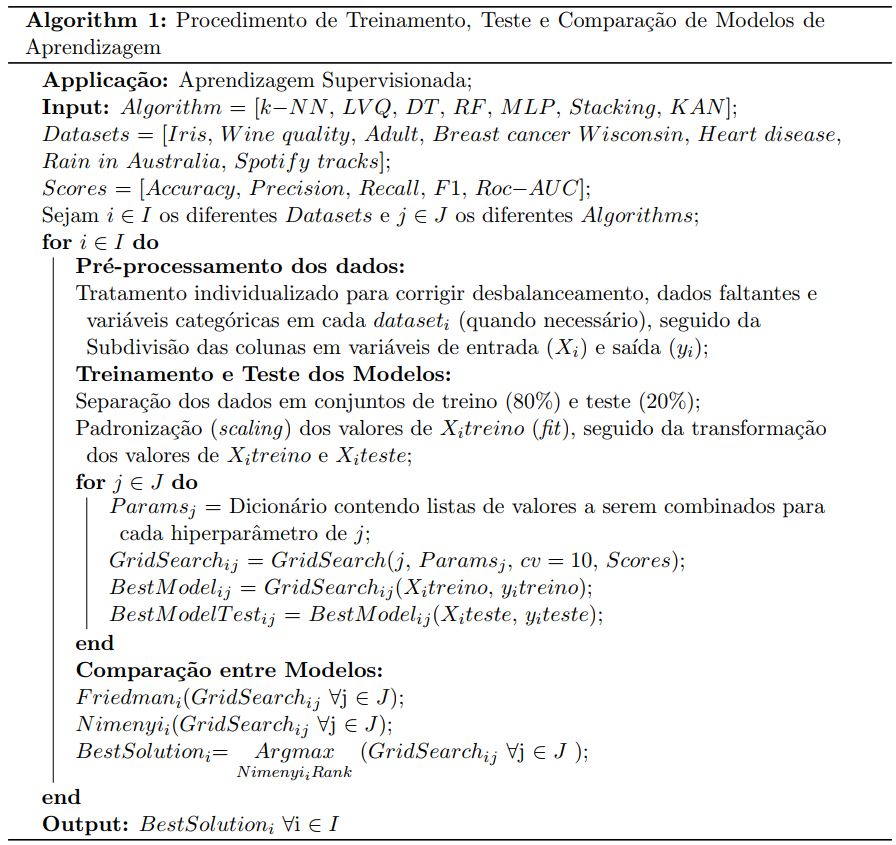
\includegraphics[width=0.9 \textwidth]{Figures/Fig3.png}
%    \caption{Exemplo da abordagem para simplificação e simbolificação de uma \textit{KAN} (LIU \textit{et al.} \cite{liu}).}
%    \label{fig:3}
%\end{figure*}

%Liu \textit{et al.} \cite{liu} avaliaram em um \textit{toy problem} que uma \textit{KAN} com arquitetura [2,1,1] apresentou melhores resultados que uma \textit{KAN} com arquitetura [2,5,1]. Já em um experimento comparando a capacidade de ajuste de funções entre \textit{KANs} e \textit{MLPs} considerando a fronteira de Pareto dada pelo número de parâmetros do modelo e pela perda de \textit{RMSE}, as \textit{KANs} apresentaram melhores fronteiras para todas as funções conforme apresentado na Figura \ref{fig:4}.


%\begin{figure*}
%    \centering
%    \includegraphics[width=0.9 \textwidth]{Figures/Fig4.png}
%    \caption{Ajuste de funções com \textit{KANs} e \textit{MLPs} para uma frente de Pareto determinada pelo número de parâmetros do modelo e pela perda de \textit{RMSE} (LIU \textit{et al.} \cite{liu}).}
%    \label{fig:4}
%\end{figure*}

%Em outro exemplo apresentado por Liu \textit{et al.} \cite{liu}, ao resolver \textit{PDEs}, uma \textit{KAN} de 2 camadas com largura de 10 mostrou-se 100 vezes mais precisa do que uma \textit{MLP} de 4 camadas com largura de 100 ($10^{-7}$ vs. $10^{-5}$ \textit{MSE}) e 100 vezes mais eficiente em termos de parâmetros ($10^{2}$ versus $10^{4}$ parâmetros). Teórica e empiricamente, as \textit{KANs} possuem leis de escala neural mais rápidas do que as \textit{MLPs}, conforme demonstrado pelos autores, além de possibilitar uma visualização intuitiva e interação com usuários humanos, tornando-as, portanto, uma abordagem com grande potencial de uso.
%===========================================================
%===========================================================
%===========================================================
%===========================================================
%==============      FIM DO DOCUMENTO       ================
%===========================================================
%===========================================================
%===========================================================
%===========================================================
%===========================================================

%\hfill mds

%\hfill August 26, 2015

%\subsection{Subsection Heading Here}
%5Subsection text here.

% needed in second column of first page if using \IEEEpubid
%\IEEEpubidadjcol

%\subsubsection{Subsubsection Heading Here}
%Subsubsection text here.


% An example of a floating figure using the graphicx package.
% Note that \label must occur AFTER (or within) \caption.
% For figures, \caption should occur after the \includegraphics.
% Note that IEEEtran v1.7 and later has special internal code that
% is designed to preserve the operation of \label within \caption
% even when the captionsoff option is in effect. However, because
% of issues like this, it may be the safest practice to put all your
% \label just after \caption rather than within \caption{}.
%
% Reminder: the "draftcls" or "draftclsnofoot", not "draft", class
% option should be used if it is desired that the figures are to be
% displayed while in draft mode.
%
%\begin{figure}[!t]
%\centering
%\includegraphics[width=2.5in]{myfigure}
% where an .eps filename suffix will be assumed under latex, 
% and a .pdf suffix will be assumed for pdflatex; or what has been declared
% via \DeclareGraphicsExtensions.
%\caption{Simulation results for the network.}
%\label{fig_sim}
%\end{figure}

% Note that the IEEE typically puts floats only at the top, even when this
% results in a large percentage of a column being occupied by floats.


% An example of a double column floating figure using two subfigures.
% (The subfig.sty package must be loaded for this to work.)
% The subfigure \label commands are set within each subfloat command,
% and the \label for the overall figure must come after \caption.
% \hfil is used as a separator to get equal spacing.
% Watch out that the combined width of all the subfigures on a 
% line do not exceed the text width or a line break will occur.
%
%\begin{figure*}[!t]
%\centering
%\subfloat[Case I]{\includegraphics[width=2.5in]{box}%
%\label{fig_first_case}}
%\hfil
%\subfloat[Case II]{\includegraphics[width=2.5in]{box}%
%\label{fig_second_case}}
%\caption{Simulation results for the network.}
%\label{fig_sim}
%\end{figure*}
%
% Note that often IEEE papers with subfigures do not employ subfigure
% captions (using the optional argument to \subfloat[]), but instead will
% reference/describe all of them (a), (b), etc., within the main caption.
% Be aware that for subfig.sty to generate the (a), (b), etc., subfigure
% labels, the optional argument to \subfloat must be present. If a
% subcaption is not desired, just leave its contents blank,
% e.g., \subfloat[].


% An example of a floating table. Note that, for IEEE style tables, the
% \caption command should come BEFORE the table and, given that table
% captions serve much like titles, are usually capitalized except for words
% such as a, an, and, as, at, but, by, for, in, nor, of, on, or, the, to
% and up, which are usually not capitalized unless they are the first or
% last word of the caption. Table text will default to \footnotesize as
% the IEEE normally uses this smaller font for tables.
% The \label must come after \caption as always.
%
%\begin{table}[!t]
%% increase table row spacing, adjust to taste
%\renewcommand{\arraystretch}{1.3}
% if using array.sty, it might be a good idea to tweak the value of
% \extrarowheight as needed to properly center the text within the cells
%\caption{An Example of a Table}
%\label{table_example}
%\centering
%% Some packages, such as MDW tools, offer better commands for making tables
%% than the plain LaTeX2e tabular which is used here.
%\begin{tabular}{|c||c|}
%\hline
%One & Two\\
%\hline
%Three & Four\\
%\hline
%\end{tabular}
%\end{table}


% Note that the IEEE does not put floats in the very first column
% - or typically anywhere on the first page for that matter. Also,
% in-text middle ("here") positioning is typically not used, but it
% is allowed and encouraged for Computer Society conferences (but
% not Computer Society journals). Most IEEE journals/conferences use
% top floats exclusively. 
% Note that, LaTeX2e, unlike IEEE journals/conferences, places
% footnotes above bottom floats. This can be corrected via the
% \fnbelowfloat command of the stfloats package.




%\section{Conclusion}
%The conclusion goes here.





% if have a single appendix:
%\appendix[Proof of the Zonklar Equations]
% or
%\appendix  % for no appendix heading
% do not use \section anymore after \appendix, only \section*
% is possibly needed

% use appendices with more than one appendix
% then use \section to start each appendix
% you must declare a \section before using any
% \subsection or using \label (\appendices by itself
% starts a section numbered zero.)
%


%\appendices
%\section{Proof of the First Zonklar Equation}
%Appendix one text goes here.

% you can choose not to have a title for an appendix
% if you want by leaving the argument blank
%\section{}
%5Appendix two text goes here.


% use section* for acknowledgment
%\section*{Acknowledgment}


%The authors would like to thank...


% Can use something like this to put references on a page
% by themselves when using endfloat and the captionsoff option.
\ifCLASSOPTIONcaptionsoff
	\newpage
\fi



% trigger a \newpage just before the given reference
% number - used to balance the columns on the last page
% adjust value as needed - may need to be readjusted if
% the document is modified later
%\IEEEtriggeratref{8}
% The "triggered" command can be changed if desired:
%\IEEEtriggercmd{\enlargethispage{-5in}}

% references section

% can use a bibliography generated by BibTeX as a .bbl file
% BibTeX documentation can be easily obtained at:
% http://mirror.ctan.org/biblio/bibtex/contrib/doc/
% The IEEEtran BibTeX style support page is at:
% http://www.michaelshell.org/tex/ieeetran/bibtex/
%\bibliographystyle{IEEEtran}
\bibliographystyle{IEEEtran}
\bibliography{./bibtex/bib/IEEEabrv,./bibtex/bib/IEEEexample}
% argument is your BibTeX string definitions and bibliography database(s)
%\bibliography{IEEEabrv,../bib/paper}
%
% <OR> manually copy in the resultant .bbl file
% set second argument of \begin to the number of references
% (used to reserve space for the reference number labels box)
%\begin{thebibliography}{1}

%\bibitem{IEEEhowto:yuanka}
%H.~Kopka and P.~W. Daly, \emph{A Guide to \LaTeX}, 3rd~ed.\hskip 1em plus
% 0.5em minus 0.4em\relax Harlow, England: Addison-Wesley, 1999.

%\end{thebibliography}

% biography section
% 
% If you have an EPS/PDF photo (graphicx package needed) extra braces are
% needed around the contents of the optional argument to biography to prevent
% the LaTeX parser from getting confused when it sees the complicated
% \includegraphics command within an optional argument. (You could create
% your own custom macro containing the \includegraphics command to make things
% simpler here.)
%\begin{IEEEbiography}[{\includegraphics[width=1in,height=1.25in,clip,keepaspectratio]{mshell}}]{Michael Shell}
% or if you just want to reserve a space for a photo:

%\begin{IEEEbiography}{Michael Shell}
%Biography text here.
%\end{IEEEbiography}

% if you will not have a photo at all:
%\begin{IEEEbiographynophoto}{John Doe}
%Biography text here.
%\end{IEEEbiographynophoto}

% insert where needed to balance the two columns on the last page with
% biographies
%\newpage

%\begin{IEEEbiographynophoto}{Jane Doe}
%Biography text here.
%\end{IEEEbiographynophoto}

% You can push biographies down or up by placing
% a \vfill before or after them. The appropriate
% use of \vfill depends on what kind of text is
% on the last page and whether or not the columns
% are being equalized.

%\vfill

% Can be used to pull up biographies so that the bottom of the last one
% is flush with the other column.
%\enlargethispage{-5in}



% that's all folks
\end{document}


